% Options for packages loaded elsewhere
\PassOptionsToPackage{unicode}{hyperref}
\PassOptionsToPackage{hyphens}{url}
\documentclass[
  ignorenonframetext,
  aspectratio=169,
]{beamer}
\newif\ifbibliography
\usepackage{pgfpages}
\setbeamertemplate{caption}[numbered]
\setbeamertemplate{caption label separator}{: }
\setbeamercolor{caption name}{fg=normal text.fg}
\beamertemplatenavigationsymbolsempty
% remove section numbering
\setbeamertemplate{part page}{
  \centering
  \begin{beamercolorbox}[sep=16pt,center]{part title}
    \usebeamerfont{part title}\insertpart\par
  \end{beamercolorbox}
}
\setbeamertemplate{section page}{
  \centering
  \begin{beamercolorbox}[sep=12pt,center]{section title}
    \usebeamerfont{section title}\insertsection\par
  \end{beamercolorbox}
}
\setbeamertemplate{subsection page}{
  \centering
  \begin{beamercolorbox}[sep=8pt,center]{subsection title}
    \usebeamerfont{subsection title}\insertsubsection\par
  \end{beamercolorbox}
}
% Prevent slide breaks in the middle of a paragraph
\widowpenalties 1 10000
\raggedbottom
\AtBeginPart{
  \frame{\partpage}
}
\AtBeginSection{
  \ifbibliography
  \else
    \frame{\sectionpage}
  \fi
}
\AtBeginSubsection{
  \frame{\subsectionpage}
}
\usepackage{iftex}
\ifPDFTeX
  \usepackage[T1]{fontenc}
  \usepackage[utf8]{inputenc}
  \usepackage{textcomp} % provide euro and other symbols
\else % if luatex or xetex
  \usepackage{unicode-math} % this also loads fontspec
  \defaultfontfeatures{Scale=MatchLowercase}
  \defaultfontfeatures[\rmfamily]{Ligatures=TeX,Scale=1}
\fi
\usepackage{lmodern}
\ifPDFTeX\else
  % xetex/luatex font selection
\fi
% Use upquote if available, for straight quotes in verbatim environments
\IfFileExists{upquote.sty}{\usepackage{upquote}}{}
\IfFileExists{microtype.sty}{% use microtype if available
  \usepackage[]{microtype}
  \UseMicrotypeSet[protrusion]{basicmath} % disable protrusion for tt fonts
}{}
\makeatletter
\@ifundefined{KOMAClassName}{% if non-KOMA class
  \IfFileExists{parskip.sty}{%
    \usepackage{parskip}
  }{% else
    \setlength{\parindent}{0pt}
    \setlength{\parskip}{6pt plus 2pt minus 1pt}}
}{% if KOMA class
  \KOMAoptions{parskip=half}}
\makeatother
\usepackage{longtable,booktabs,array}
\usepackage{caption}
\captionsetup[table]{skip=6pt}
\newcounter{none} % for unnumbered tables
\usepackage{calc} % for calculating minipage widths
\usepackage{caption}
% Make caption package work with longtable
\makeatletter
\def\fnum@table{\tablename~\thetable}
\makeatother
\usepackage{graphicx}
\makeatletter
\newsavebox\pandoc@box
\newcommand*\pandocbounded[1]{% scales image to fit in text height/width
  \sbox\pandoc@box{#1}%
  \Gscale@div\@tempa{\textheight}{\dimexpr\ht\pandoc@box+\dp\pandoc@box\relax}%
  \Gscale@div\@tempb{\linewidth}{\wd\pandoc@box}%
  \ifdim\@tempb\p@<\@tempa\p@\let\@tempa\@tempb\fi% select the smaller of both
  \ifdim\@tempa\p@<\p@\scalebox{\@tempa}{\usebox\pandoc@box}%
  \else\usebox{\pandoc@box}%
  \fi%
}
% Set default figure placement to htbp
\def\fps@figure{htbp}
\makeatother
\setlength{\emergencystretch}{3em} % prevent overfull lines
\providecommand{\tightlist}{%
  \setlength{\itemsep}{0pt}\setlength{\parskip}{0pt}}
% Auto-generated by infrastructure/rendering/_pdf_latex_helpers.py::extract_math_font_preamble.
% Minimal header passed to Pandoc via -H so Beamer slides pick up the same math font
% as the combined-PDF path. Adjust the manuscript's preamble.md to change the font globally.
\usepackage{unicode-math}
\setmathfont{latinmodern-math.otf}

% Manuscript macro/package fallbacks (newcommand -> providecommand).
% Core mathematics
\usepackage{amsmath}
\usepackage{amssymb}
% Document layout
% Tables
\usepackage{booktabs}
% Caption styling (booktabs already loaded above). Small caption font with a
% bold label ("Figure 1", "Table 2") gives the math/figure-heavy layout a
% consistent, journal-like caption rhythm without fighting pandoc-crossref —
% pandoc emits standard \caption{}, and caption/captionsetup only restyle it.
% ── Theorem environments ─────────────────────────────────────────────────
% amsthm is loaded above. The FedGVI<->Friston bridge is stated as a small
% number of theorems/definitions/lemmas/propositions/corollaries; sharing one
% counter (definition/lemma/proposition/corollary all step the `theorem`
% counter) gives a single monotone numbering 1, 2, 3, ... across all kinds, so
% authors can reference them as Theorem 1, Definition 2, Corollary 3 without a
% per-kind counter drifting out of order. Plain style for theorem-like results,
% definition style (upright body) for definitions.
% (algorithm2e intentionally not loaded: this manuscript states results as
% numbered amsthm Theorems/Definitions, not algorithm2e pseudocode.)
% Code listings
\usepackage{listings}
% Typography and formatting
% (siunitx intentionally not loaded: no \SI/\num units appear in this manuscript.)
% Cross-references and citations
% (cleveref and titlesec intentionally not loaded: unavailable in this TeX tree
% and not required. Cross-references resolve through pandoc-crossref's own
% \ref-style names — no \cref appears — and section heading styling falls back
% to the pandoc/LaTeX defaults.)
% ── TeX Live Basic-compatible mono font for code listings ────────────
% Latin Modern Mono is bundled with TeX Live Basic and keeps the manuscript
% renderable on minimal TeX installations. Mathematical Unicode coverage is
% provided separately by Latin Modern Math below, so the code font does not
% need a private JuliaMono installation.
%
% Use the TeX font filename rather than the system-family name: the minimal
% TeX Live fontconfig database may not register the OpenType family even though
% kpsewhich can resolve the bundled files.
% Math font for unicode-math: Latin Modern Math (TeX Live) has full BMP
% coverage including U+2223 (\mid), U+226A/226B (\ll/\gg), and the Greek/
% blackboard letters used in equations. Without an explicit \setmathfont,
% unicode-math falls back to lmroman text font which lacks several glyphs
% and emits "Missing character" warnings on every \mid in math mode.

% Slide layout defaults for warning-clean scientific decks.
\usepackage{etoolbox}
\IfFileExists{xurl.sty}{\usepackage{xurl}}{}
\IfFileExists{seqsplit.sty}{\usepackage{seqsplit}}{\newcommand{\seqsplit}[1]{#1}}
\protected\def\breakseq#1{\seqsplit{#1}}
\protected\def\breaktt#1{\begingroup\ttfamily\seqsplit{#1}\endgroup}
\setlength{\emergencystretch}{6em}
\tolerance=5000
\hbadness=10000
\hfuzz=1pt
\setlength{\tabcolsep}{2pt}
\AtBeginEnvironment{longtable}{\tiny\renewcommand{\arraystretch}{0.86}\setlength{\tabcolsep}{1pt}}
\AtBeginEnvironment{tabular}{\tiny\renewcommand{\arraystretch}{0.86}\setlength{\tabcolsep}{1pt}}
\AtBeginEnvironment{equation}{\tiny}
\AtBeginEnvironment{equation*}{\tiny}
\AtBeginEnvironment{align}{\tiny}
\AtBeginEnvironment{align*}{\tiny}
\AtBeginEnvironment{itemize}{\footnotesize}
\AtBeginEnvironment{enumerate}{\footnotesize}
\AtBeginEnvironment{description}{\footnotesize}
\setbeamerfont{caption}{size=\tiny}
\setbeamerfont{caption name}{size=\tiny}
\setbeamerfont{normal text}{size=\small}
\setbeamerfont{frametitle}{size=\small}
\setbeamerfont{section title}{size=\footnotesize}
\setbeamerfont{subsection title}{size=\footnotesize}
\setbeamertemplate{section page}{%
  \centering
  \begin{beamercolorbox}[sep=12pt,center,wd=\paperwidth]{section title}
    \parbox{0.86\paperwidth}{\centering\usebeamerfont{section title}\insertsection\par}
  \end{beamercolorbox}
}
\setbeamertemplate{subsection page}{%
  \centering
  \begin{beamercolorbox}[sep=8pt,center,wd=\paperwidth]{subsection title}
    \parbox{0.86\paperwidth}{\centering\usebeamerfont{subsection title}\insertsubsection\par}
  \end{beamercolorbox}
}
\setlength{\abovecaptionskip}{2pt}
\setlength{\belowcaptionskip}{0pt}

% Natbib and cross-reference fallbacks — slides don't load natbib
% or cleveref, but combined-PDF manuscript prose may emit these
% commands. The fallback renders citations as a bracketed key list
% and cross-references as detokenized labels so slides don't fail on
% undefined control sequences or raw underscores. \providecommand is
% a no-op if packages load later.
\providecommand{\citep}[1]{[#1]}
\providecommand{\citet}[1]{#1}
\providecommand{\citealp}[1]{#1}
\providecommand{\citeauthor}[1]{#1}
\providecommand{\citeyear}[1]{#1}
\providecommand{\cref}[1]{\texttt{\detokenize{#1}}}
\providecommand{\Cref}[1]{\texttt{\detokenize{#1}}}
\providecommand{\crefrange}[2]{\texttt{\detokenize{#1}}--\texttt{\detokenize{#2}}}
\providecommand{\Crefrange}[2]{\texttt{\detokenize{#1}}--\texttt{\detokenize{#2}}}
\providecommand{\paragraph}[1]{\textbf{#1}\ }

% Opt-in accessible presentation profile.
\setbeamerfont{normal text}{size*={20pt}{24pt}}
\setbeamerfont{frametitle}{size*={28pt}{32pt}}
\setbeamerfont{section title}{size*={28pt}{32pt}}
\setbeamerfont{subsection title}{size*={28pt}{32pt}}
\setbeamerfont{caption}{size*={16pt}{19pt}}
\setbeamerfont{caption name}{size*={16pt}{19pt}}
\setbeamerfont{itemize/enumerate body}{size*={20pt}{24pt}}
\setbeamerfont{itemize/enumerate subbody}{size*={20pt}{24pt}}
\setbeamerfont{itemize/enumerate subsubbody}{size*={20pt}{24pt}}
\setbeamerfont{itemize item}{size*={20pt}{24pt}}
\setbeamerfont{itemize subitem}{size*={20pt}{24pt}}
\setbeamerfont{itemize subsubitem}{size*={20pt}{24pt}}
\setbeamerfont{description body}{size*={20pt}{24pt}}
\setbeamerfont{description item}{size*={20pt}{24pt}}
\setbeamerfont{quote}{size*={20pt}{24pt}}
\setbeamerfont{quotation}{size*={20pt}{24pt}}
\AtBeginEnvironment{longtable}{\fontsize{20pt}{24pt}\selectfont}
\AtBeginEnvironment{tabular}{\fontsize{20pt}{24pt}\selectfont}
\AtBeginEnvironment{equation}{\fontsize{20pt}{24pt}\selectfont}
\AtBeginEnvironment{equation*}{\fontsize{20pt}{24pt}\selectfont}
\AtBeginEnvironment{align}{\fontsize{20pt}{24pt}\selectfont}
\AtBeginEnvironment{align*}{\fontsize{20pt}{24pt}\selectfont}
\AtBeginEnvironment{itemize}{\fontsize{20pt}{24pt}\selectfont}
\AtBeginEnvironment{enumerate}{\fontsize{20pt}{24pt}\selectfont}
\AtBeginEnvironment{description}{\fontsize{20pt}{24pt}\selectfont}
\AtBeginDocument{\usebeamerfont{normal text}}
\newlength{\AFSlideTableWidth}
% The fixed footer reservation is calibrated with the semantic seven-line regular-body budget.
\setbeamertemplate{footline}{%
  \leavevmode\vbox{%
    \hbox{%
      \begin{beamercolorbox}[wd=\paperwidth,ht=16pt,dp=3pt,center]{author in head/foot}%
        \fontsize{16pt}{19pt}\selectfont Untagged PDF derivative \textbar\ \href{../web/index.html}{HTML reader}%
      \end{beamercolorbox}%
    }%
    \vskip6pt%
  }%
}
% Accessible footer reserved height: 25pt.

\newtheorem{proposition}{Proposition}
\newtheorem{hypothesis}{Hypothesis}
\newtheorem{remark}[theorem]{Remark}
\newtheorem{axiom}{Axiom}
\newtheorem{property}{Property}
\usepackage{bookmark}
\IfFileExists{xurl.sty}{\usepackage{xurl}}{} % add URL line breaks if available
\urlstyle{same}
% fallback for those not using the hyperref driver hyperxmp:
\makeatletter
\@ifundefined{xmpquote}{\newcommand{\xmpquote}[1]{#1}}{}
\makeatother
\hypersetup{
  hidelinks,
  pdfcreator={LaTeX via pandoc}}

\author{\texorpdfstring{}{}}
\date{}

\begin{document}

\section{Reproducibility: producer provenance and recovery
checks}\label{sec:repro-production}

\begin{frame}{Producer order, stale invalidation, and publication
authority}
\protect\phantomsection\label{sec:repro-provenance-map}
The provenance map in fig.~20 records
the source-owned producer contract rather than inferring it from the
release manifest.
\end{frame}

\begin{frame}{Producer order, stale\ldots{} (part 2)}
Panel A places the non-sequential fan-in dependencies in a labeled
matrix, then orders the temporal, gate, receipt, and authorization
dependencies in a crossing-free process path. Source, configuration,
lockfile,
\end{frame}

\begin{frame}{Producer order, stale\ldots{} (part 3)}
figure-accessibility registries, and the exact clean Template commit
remain explicit inputs.
\end{frame}

\begin{frame}{Producer order, stale\ldots{} (part 4)}
Panel B's fourteen coded dashed cards make reverse invalidation explicit
without crossing the forward process path. Each arrow starts at one or
more immediate stale targets on the right and points back to its changed
owner on the left.
\end{frame}

\begin{frame}{Producer order, stale\ldots{} (part 5)}
A changed owner makes the named immediate targets and their downstream
reports, figures, hydrated text, rendered surfaces, provenance, and
release receipts stale; previously green bytes are not carried forward.
\end{frame}

\begin{frame}{Producer order, stale\ldots{} (part 6)}
GitHub and Zenodo are terminal authorization states, not automatic
products of a green build. The figure itself is generated from the
source-owned pipeline contract and never reads the downstream release
manifest that later inventories it, avoiding a circular dependency.
\end{frame}

\begin{frame}{Producer order, stale\ldots{} (part 7)}
\begin{figure}
\centering
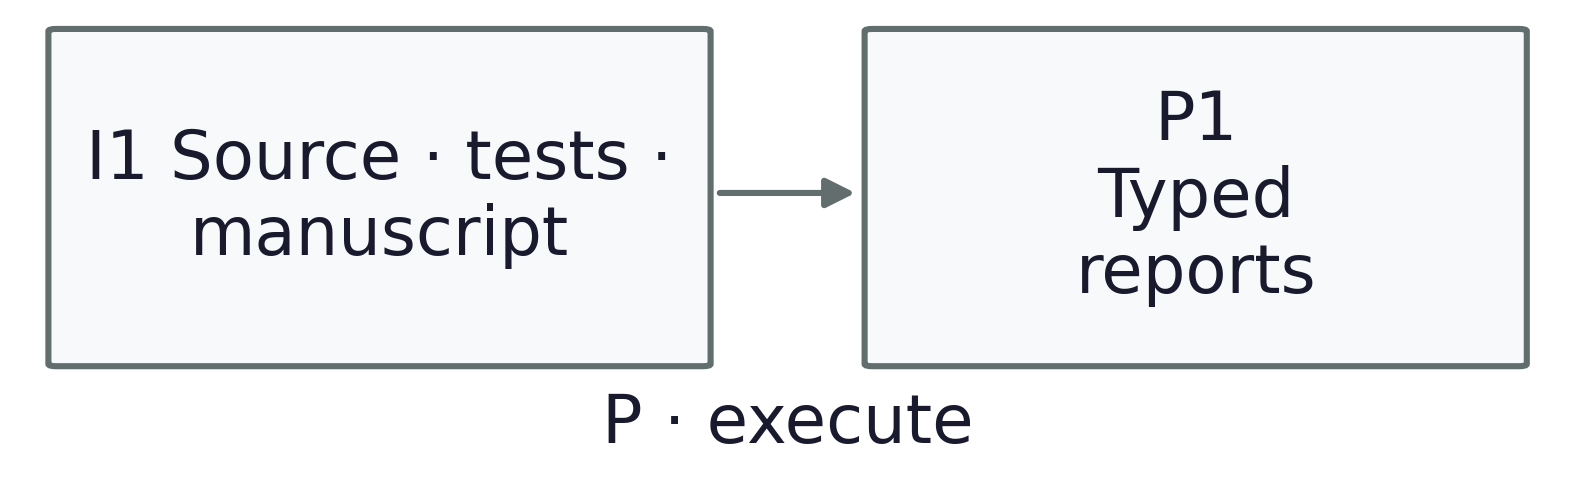
\includegraphics[keepaspectratio,width=0.98\linewidth,height=0.8\textheight,alt={I1  Source · tests · manuscript → P1 Typed reports: P · execute; producer.}]{../figures/source_render_provenance.slide-producer-source-reports.png}
\refstepcounter{figure}\label{fig:source-render-provenance-slide-panel-1}
\end{figure}
\end{frame}

\begin{frame}{Producer order, stale\ldots{} (part 8)}
\begin{figure}
\centering
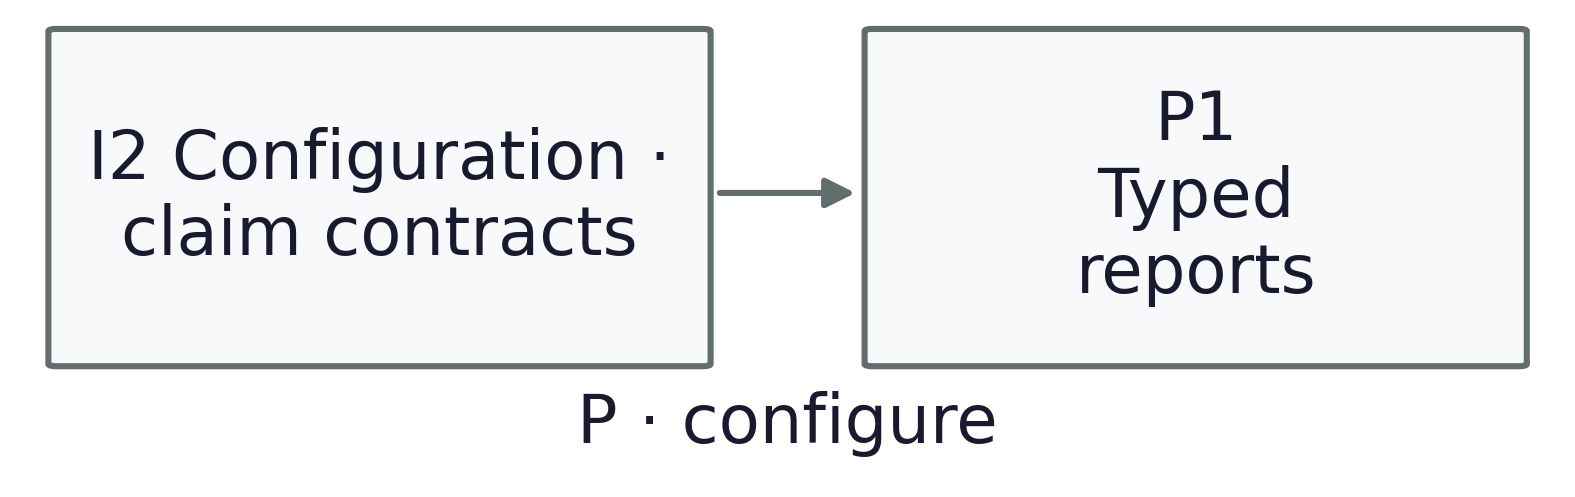
\includegraphics[keepaspectratio,width=0.98\linewidth,height=0.8\textheight,alt={I2  Configuration · claim contracts → P1 Typed reports: P · configure; producer.}]{../figures/source_render_provenance.slide-producer-config-reports.png}
\refstepcounter{figure}\label{fig:source-render-provenance-slide-panel-2}
\end{figure}
\end{frame}

\begin{frame}{Producer order, stale\ldots{} (part 9)}
\begin{figure}
\centering
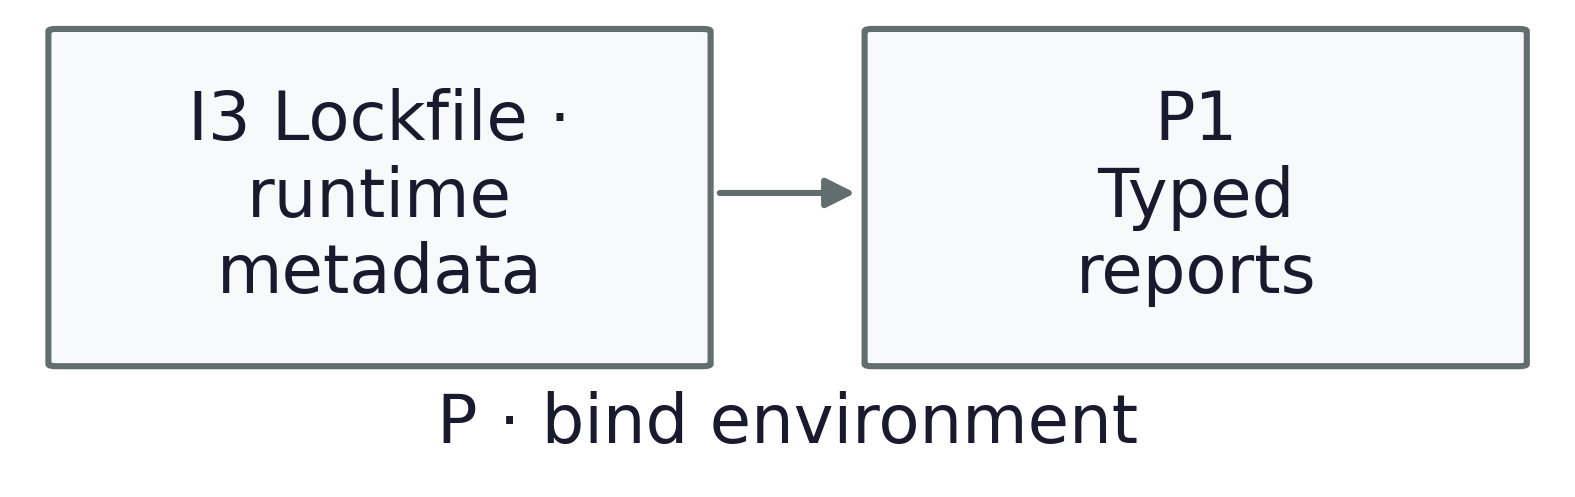
\includegraphics[keepaspectratio,width=0.98\linewidth,height=0.8\textheight,alt={I3  Lockfile · runtime metadata → P1 Typed reports: P · bind environment; producer.}]{../figures/source_render_provenance.slide-producer-lockfile-reports.png}
\refstepcounter{figure}\label{fig:source-render-provenance-slide-panel-3}
\end{figure}
\end{frame}

\begin{frame}{Producer order, stale\ldots{} (part 10)}
\begin{figure}
\centering
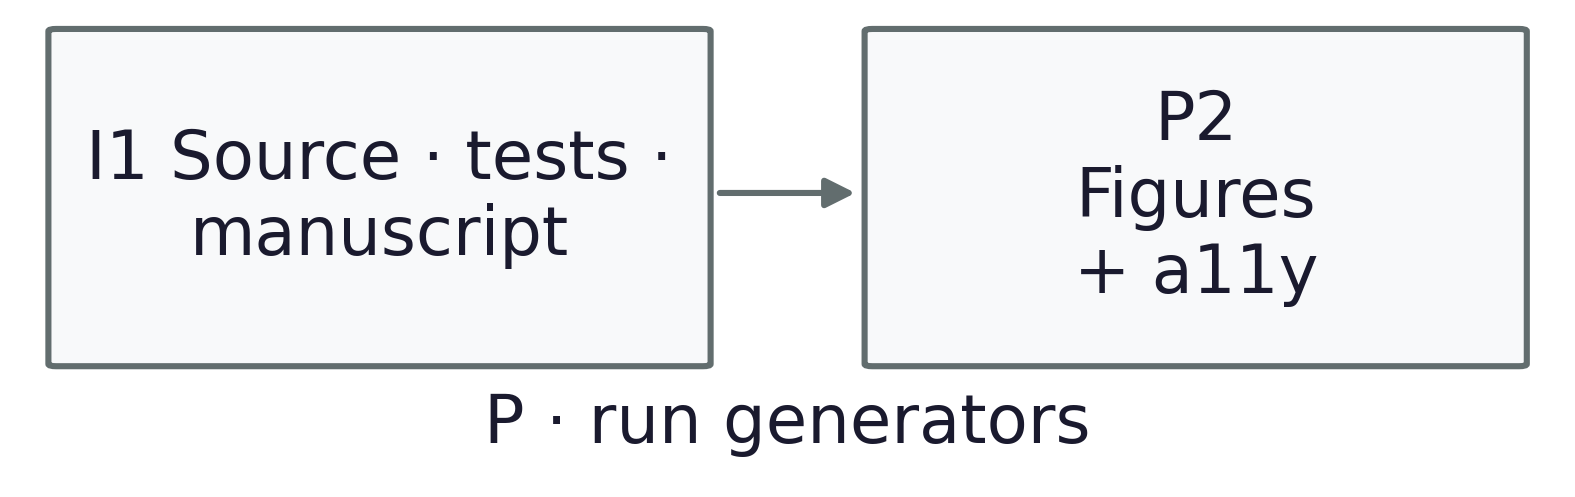
\includegraphics[keepaspectratio,width=0.98\linewidth,height=0.8\textheight,alt={I1  Source · tests · manuscript → P2 Figures + a11y: P · run generators; producer.}]{../figures/source_render_provenance.slide-producer-source-figures.png}
\refstepcounter{figure}\label{fig:source-render-provenance-slide-panel-4}
\end{figure}
\end{frame}

\begin{frame}{Producer order, stale\ldots{} (part 11)}
\begin{figure}
\centering
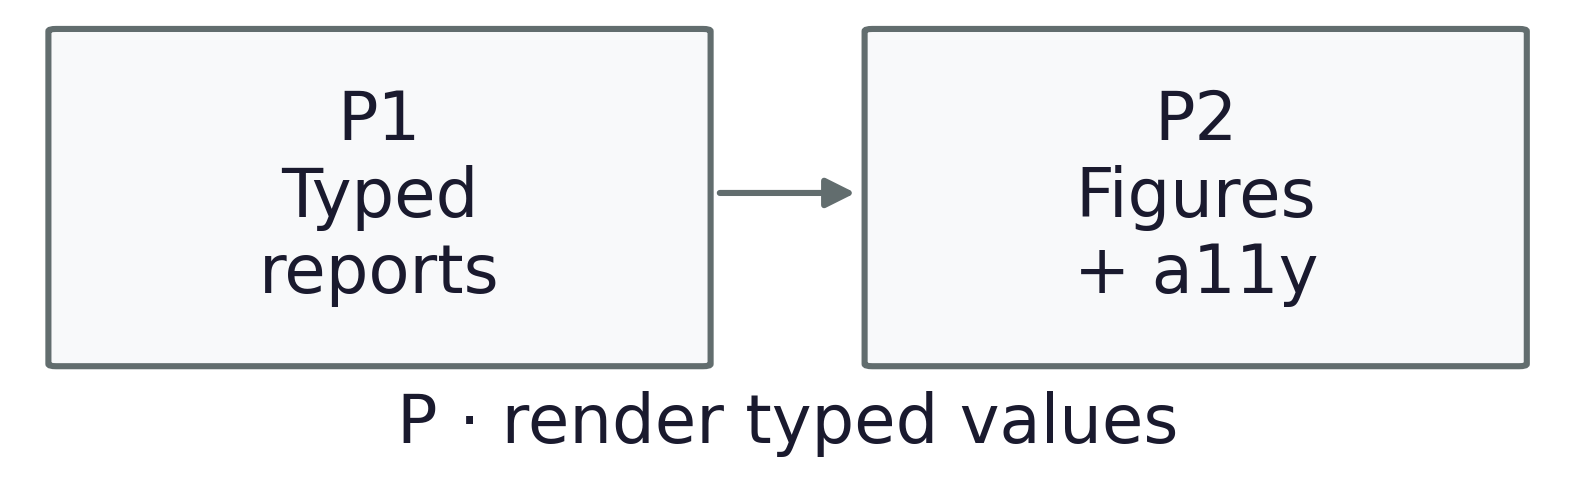
\includegraphics[keepaspectratio,width=0.98\linewidth,height=0.8\textheight,alt={P1 Typed reports → P2 Figures + a11y: P · render typed values; producer.}]{../figures/source_render_provenance.slide-producer-reports-figures.png}
\refstepcounter{figure}\label{fig:source-render-provenance-slide-panel-5}
\end{figure}
\end{frame}

\begin{frame}{Producer order, stale\ldots{} (part 12)}
\begin{figure}
\centering
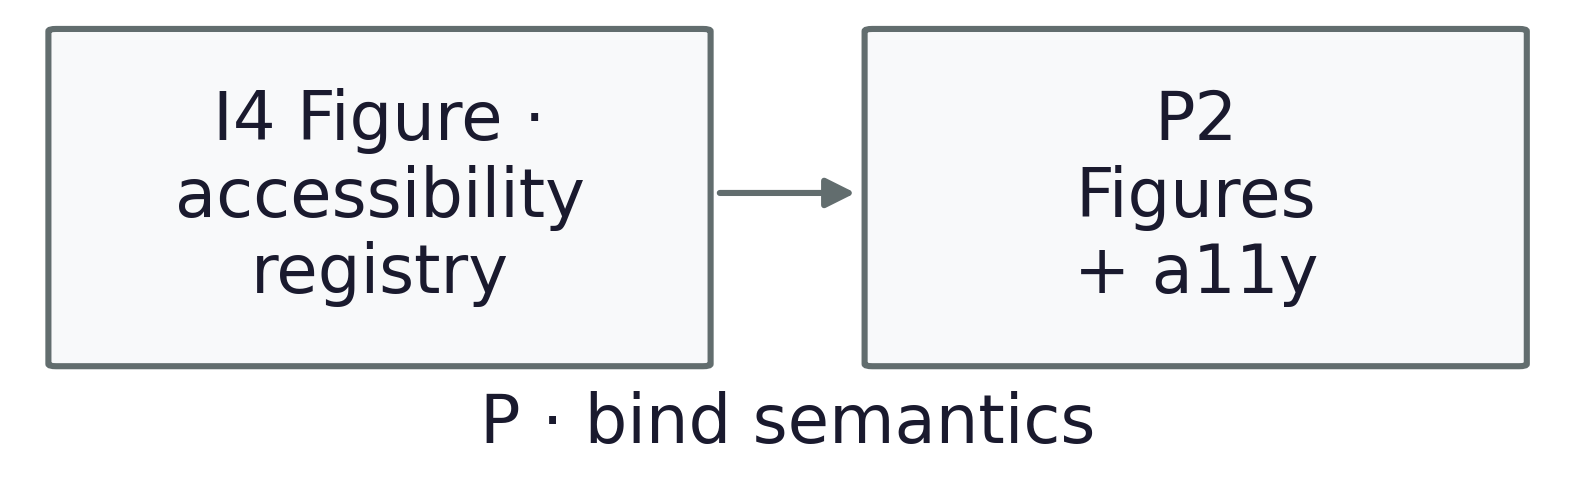
\includegraphics[keepaspectratio,width=0.98\linewidth,height=0.8\textheight,alt={I4  Figure · accessibility registry → P2 Figures + a11y: P · bind semantics; producer.}]{../figures/source_render_provenance.slide-producer-registry-figures.png}
\refstepcounter{figure}\label{fig:source-render-provenance-slide-panel-6}
\end{figure}
\end{frame}

\begin{frame}{Producer order, stale\ldots{} (part 13)}
\begin{figure}
\centering
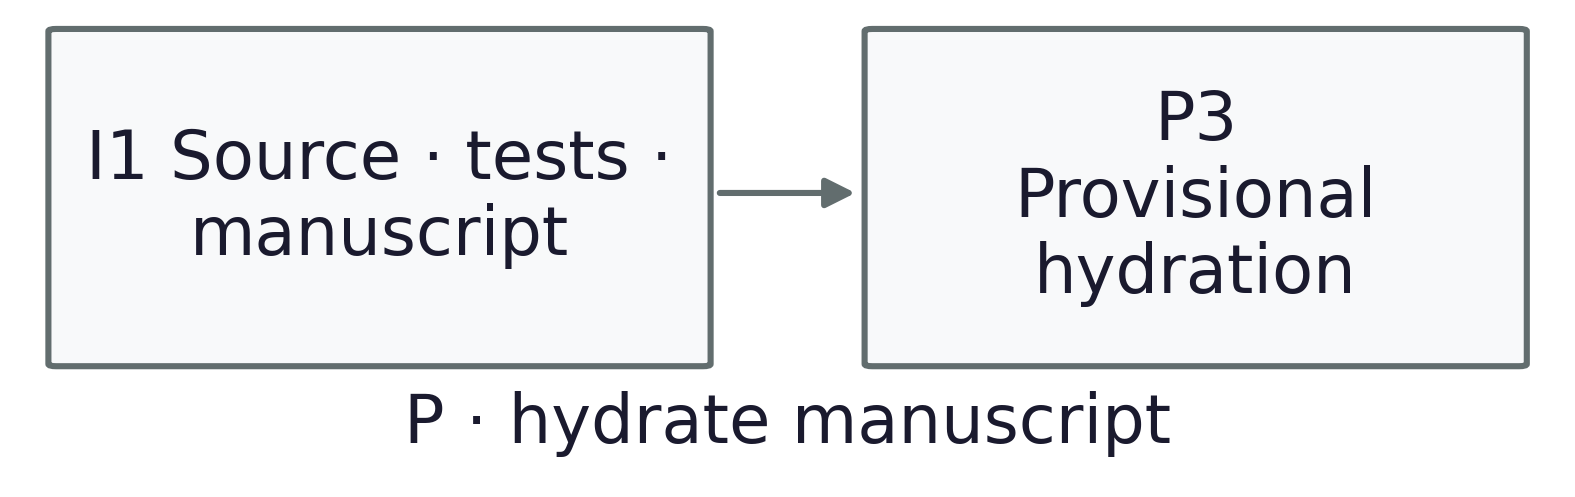
\includegraphics[keepaspectratio,width=0.98\linewidth,height=0.8\textheight,alt={I1  Source · tests · manuscript → P3 Provisional hydration: P · hydrate manuscript; producer.}]{../figures/source_render_provenance.slide-producer-source-provisional.png}
\refstepcounter{figure}\label{fig:source-render-provenance-slide-panel-7}
\end{figure}
\end{frame}

\begin{frame}{Producer order, stale\ldots{} (part 14)}
\begin{figure}
\centering
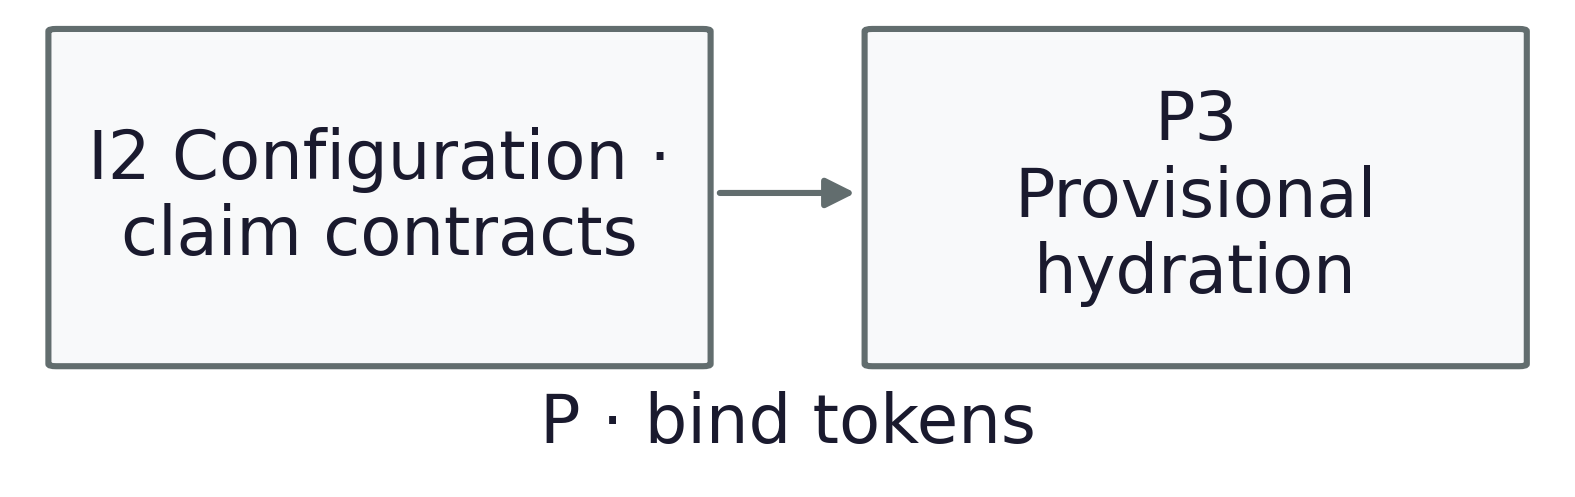
\includegraphics[keepaspectratio,width=0.98\linewidth,height=0.8\textheight,alt={I2  Configuration · claim contracts → P3 Provisional hydration: P · bind tokens; producer.}]{../figures/source_render_provenance.slide-producer-config-provisional.png}
\refstepcounter{figure}\label{fig:source-render-provenance-slide-panel-8}
\end{figure}
\end{frame}

\begin{frame}{Producer order, stale\ldots{} (part 15)}
\begin{figure}
\centering
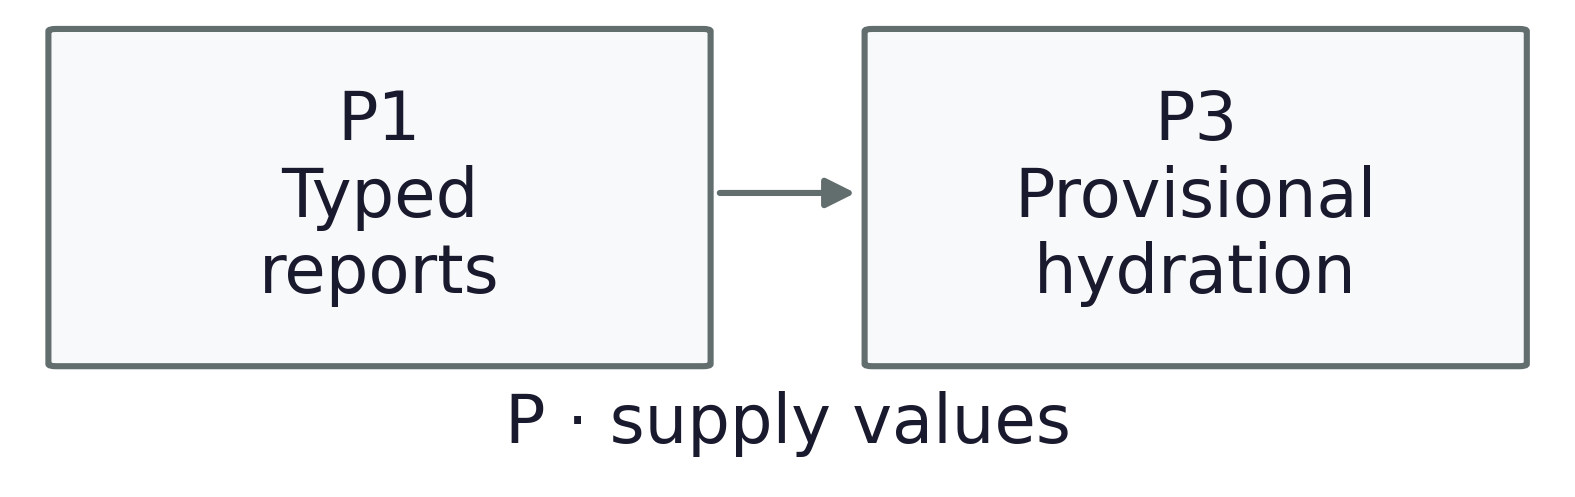
\includegraphics[keepaspectratio,width=0.98\linewidth,height=0.8\textheight,alt={P1 Typed reports → P3 Provisional hydration: P · supply values; producer.}]{../figures/source_render_provenance.slide-producer-reports-provisional.png}
\refstepcounter{figure}\label{fig:source-render-provenance-slide-panel-9}
\end{figure}
\end{frame}

\begin{frame}{Producer order, stale\ldots{} (part 16)}
\begin{figure}
\centering

\includegraphics[keepaspectratio,width=0.98\linewidth,height=0.8\textheight,alt={I1  Source · tests · manuscript → G4 Tests + coverage: G · test source; gate.}]{../figures/source_render_provenance.slide-producer-source-coverage.png}
\refstepcounter{figure}\label{fig:source-render-provenance-slide-panel-10}
\end{figure}
\end{frame}

\begin{frame}{Producer order, stale\ldots{} (part 17)}
\begin{figure}
\centering
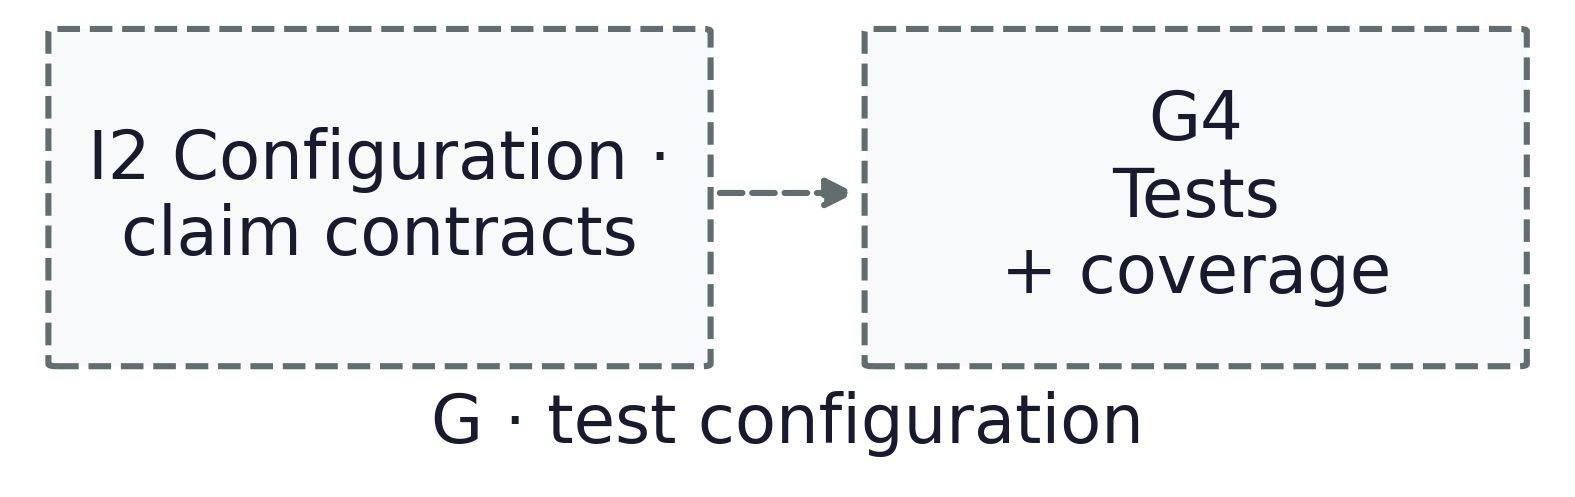
\includegraphics[keepaspectratio,width=0.98\linewidth,height=0.8\textheight,alt={I2  Configuration · claim contracts → G4 Tests + coverage: G · test configuration; gate.}]{../figures/source_render_provenance.slide-producer-config-coverage.png}
\refstepcounter{figure}\label{fig:source-render-provenance-slide-panel-11}
\end{figure}
\end{frame}

\begin{frame}{Producer order, stale\ldots{} (part 18)}
\begin{figure}
\centering
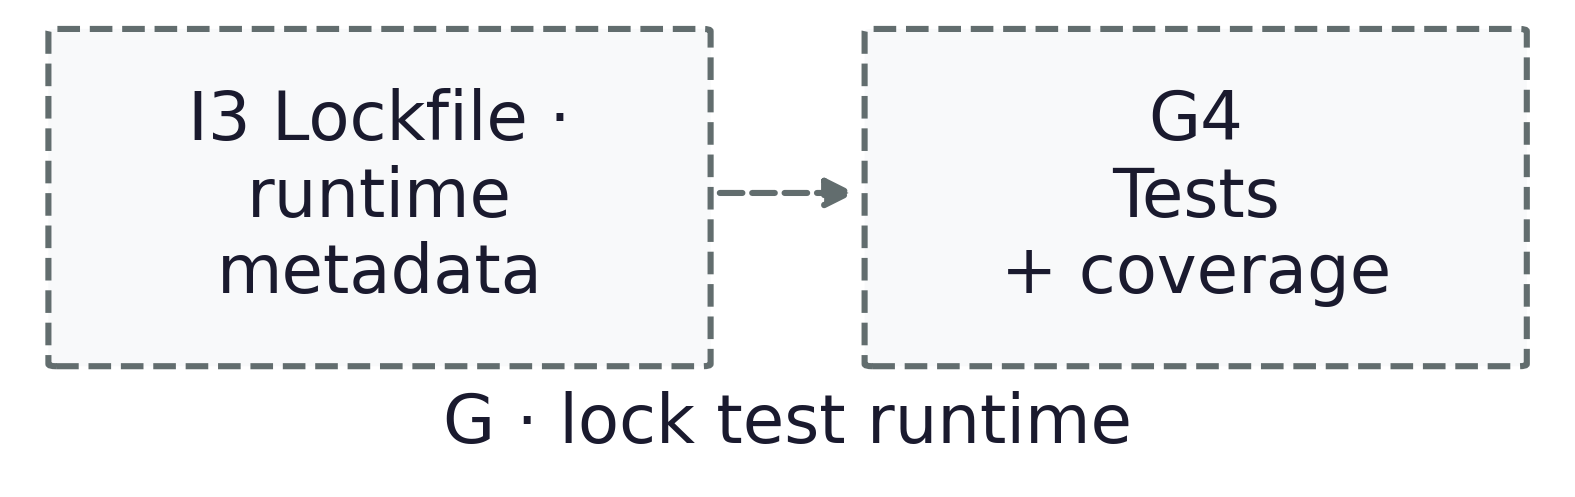
\includegraphics[keepaspectratio,width=0.98\linewidth,height=0.8\textheight,alt={I3  Lockfile · runtime metadata → G4 Tests + coverage: G · lock test runtime; gate.}]{../figures/source_render_provenance.slide-producer-lockfile-coverage.png}
\refstepcounter{figure}\label{fig:source-render-provenance-slide-panel-12}
\end{figure}
\end{frame}

\begin{frame}{Producer order, stale\ldots{} (part 19)}
\begin{figure}
\centering
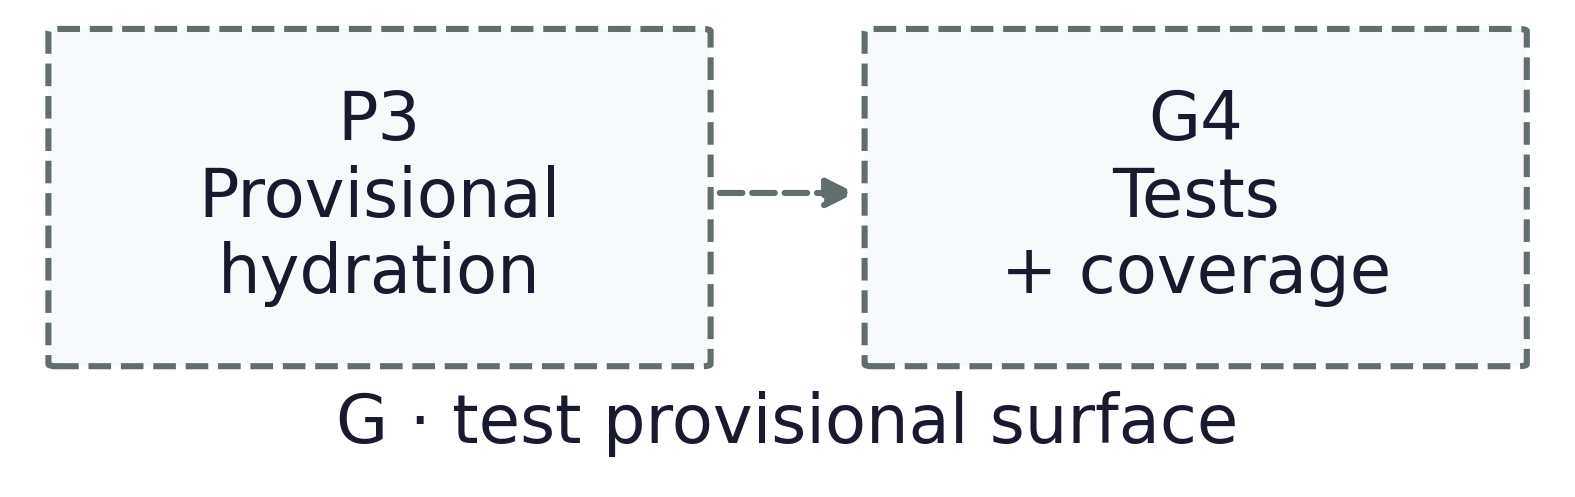
\includegraphics[keepaspectratio,width=0.98\linewidth,height=0.8\textheight,alt={P3 Provisional hydration → G4 Tests + coverage: G · test provisional surface; gate.}]{../figures/source_render_provenance.slide-producer-provisional-coverage.png}
\refstepcounter{figure}\label{fig:source-render-provenance-slide-panel-13}
\end{figure}
\end{frame}

\begin{frame}{Producer order, stale\ldots{} (part 20)}
\begin{figure}
\centering
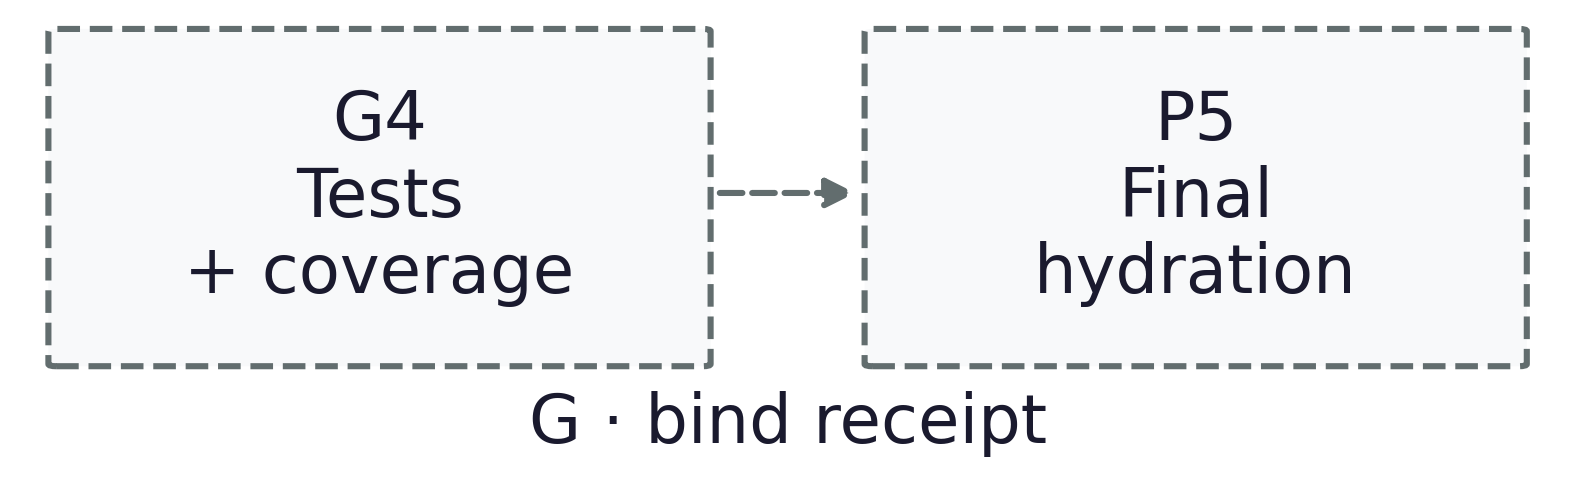
\includegraphics[keepaspectratio,width=0.98\linewidth,height=0.8\textheight,alt={G4 Tests + coverage → P5 Final hydration: G · bind receipt; gate.}]{../figures/source_render_provenance.slide-producer-coverage-final-hydration.png}
\refstepcounter{figure}\label{fig:source-render-provenance-slide-panel-14}
\end{figure}
\end{frame}

\begin{frame}{Producer order, stale\ldots{} (part 21)}
\begin{figure}
\centering
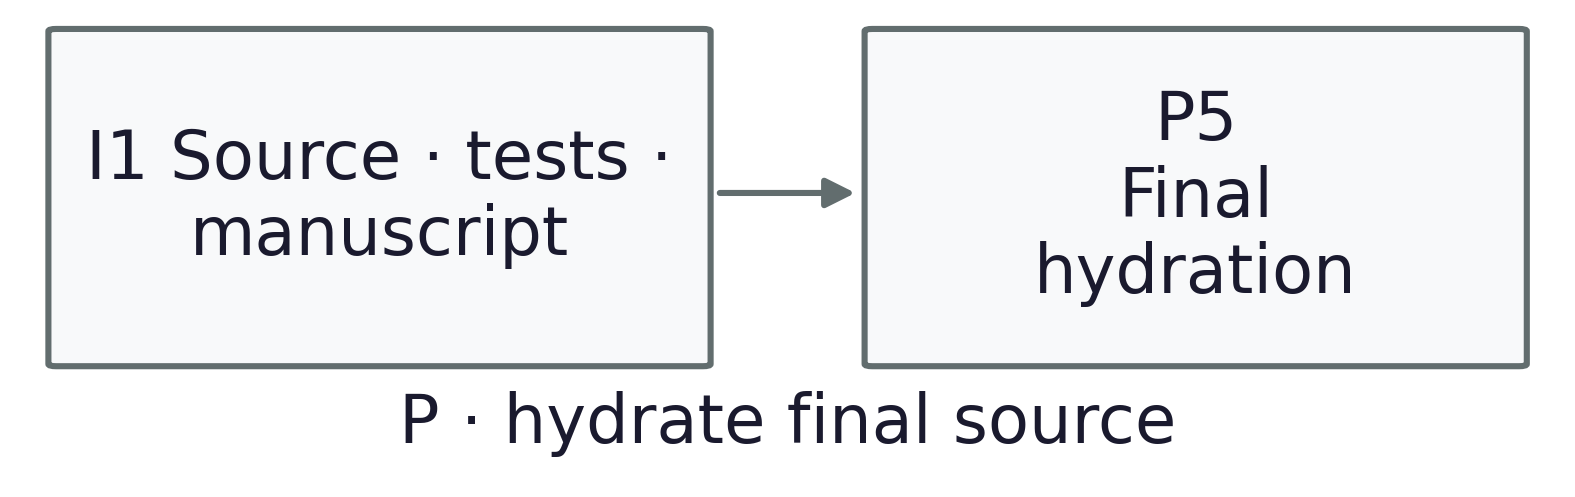
\includegraphics[keepaspectratio,width=0.98\linewidth,height=0.8\textheight,alt={I1  Source · tests · manuscript → P5 Final hydration: P · hydrate final source; producer.}]{../figures/source_render_provenance.slide-producer-source-final-hydration.png}
\refstepcounter{figure}\label{fig:source-render-provenance-slide-panel-15}
\end{figure}
\end{frame}

\begin{frame}{Producer order, stale\ldots{} (part 22)}
\begin{figure}
\centering
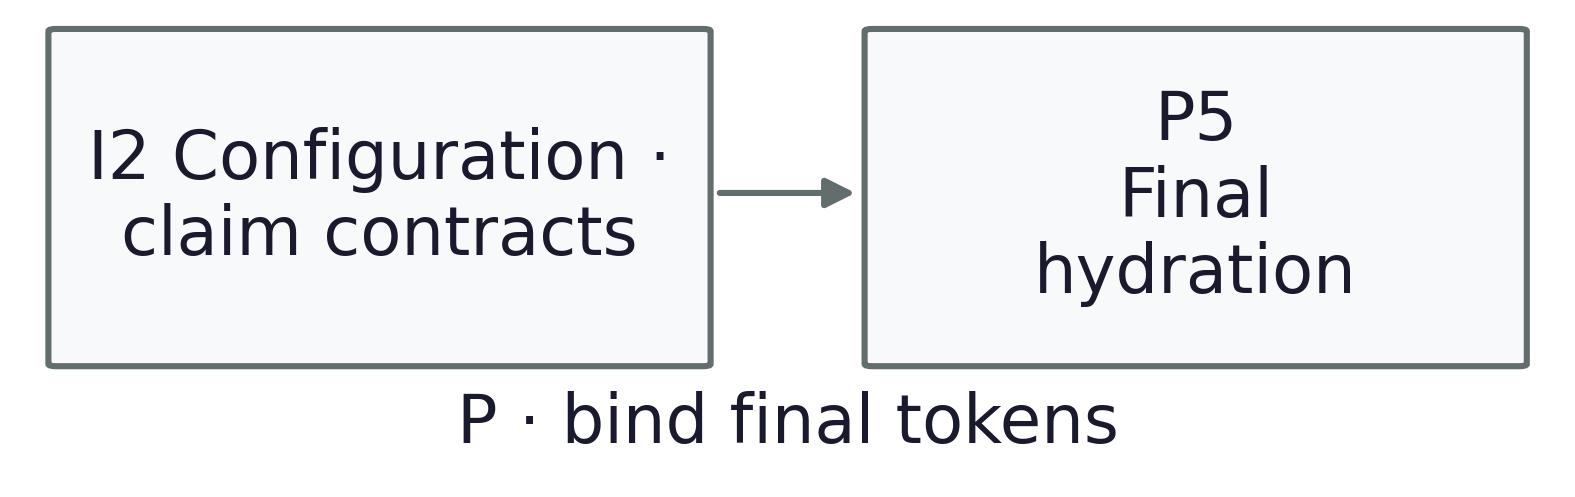
\includegraphics[keepaspectratio,width=0.98\linewidth,height=0.8\textheight,alt={I2  Configuration · claim contracts → P5 Final hydration: P · bind final tokens; producer.}]{../figures/source_render_provenance.slide-producer-config-final-hydration.png}
\refstepcounter{figure}\label{fig:source-render-provenance-slide-panel-16}
\end{figure}
\end{frame}

\begin{frame}{Producer order, stale\ldots{} (part 23)}
\begin{figure}
\centering
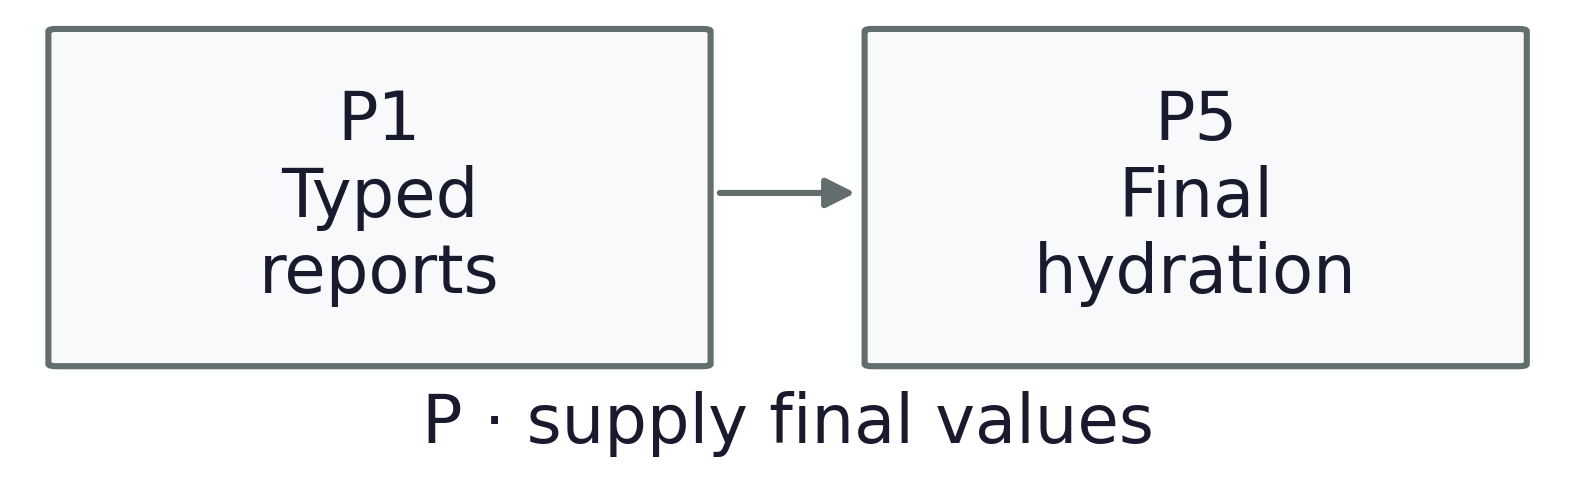
\includegraphics[keepaspectratio,width=0.98\linewidth,height=0.8\textheight,alt={P1 Typed reports → P5 Final hydration: P · supply final values; producer.}]{../figures/source_render_provenance.slide-producer-reports-final-hydration.png}
\refstepcounter{figure}\label{fig:source-render-provenance-slide-panel-17}
\end{figure}
\end{frame}

\begin{frame}{Producer order, stale\ldots{} (part 24)}
\begin{figure}
\centering
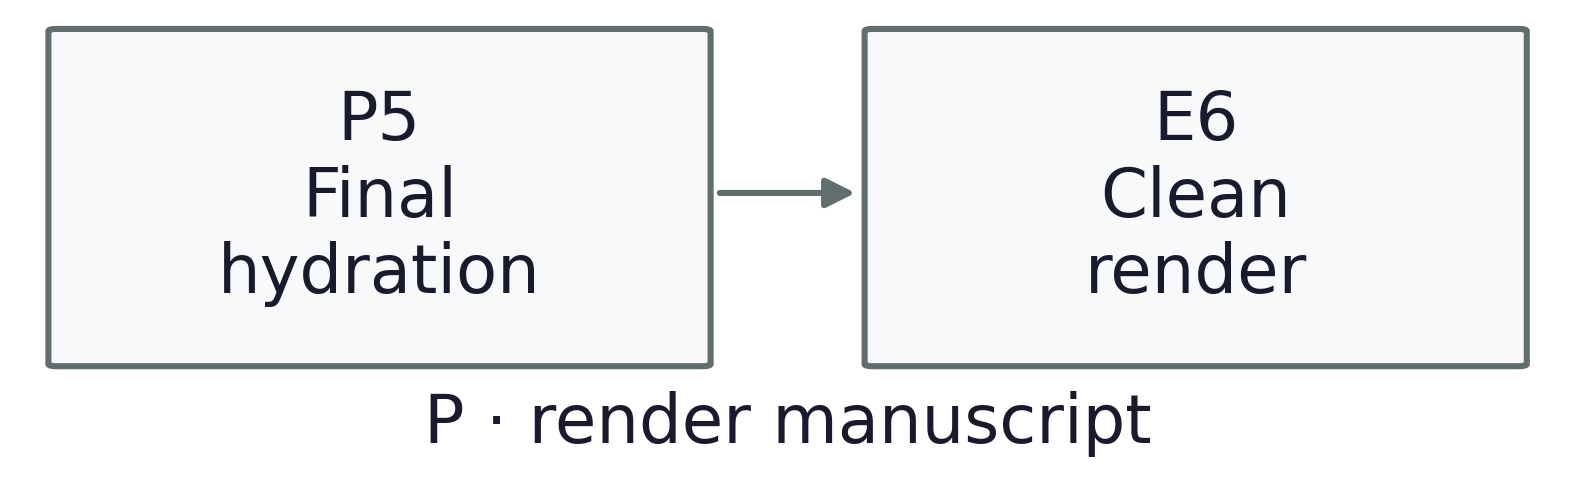
\includegraphics[keepaspectratio,width=0.98\linewidth,height=0.8\textheight,alt={P5 Final hydration → E6 Clean render: P · render manuscript; producer.}]{../figures/source_render_provenance.slide-producer-final-hydration-render.png}
\refstepcounter{figure}\label{fig:source-render-provenance-slide-panel-18}
\end{figure}
\end{frame}

\begin{frame}{Producer order, stale\ldots{} (part 25)}
\begin{figure}
\centering
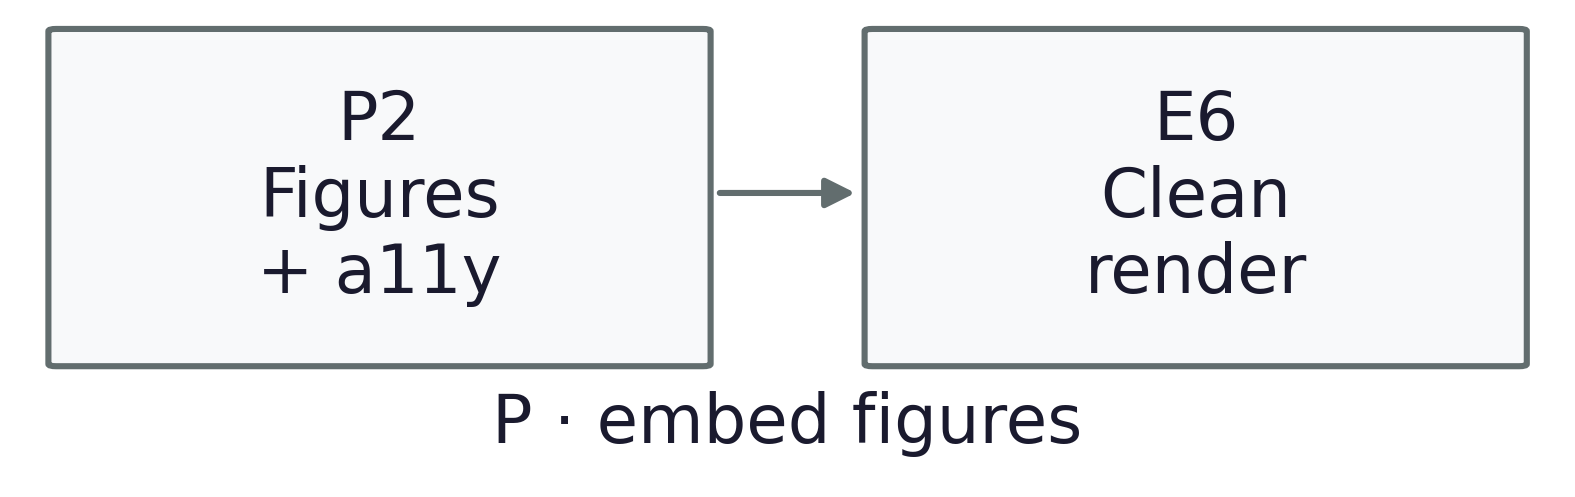
\includegraphics[keepaspectratio,width=0.98\linewidth,height=0.8\textheight,alt={P2 Figures + a11y → E6 Clean render: P · embed figures; producer.}]{../figures/source_render_provenance.slide-producer-figures-render.png}
\refstepcounter{figure}\label{fig:source-render-provenance-slide-panel-19}
\end{figure}
\end{frame}

\begin{frame}{Producer order, stale\ldots{} (part 26)}
\begin{figure}
\centering
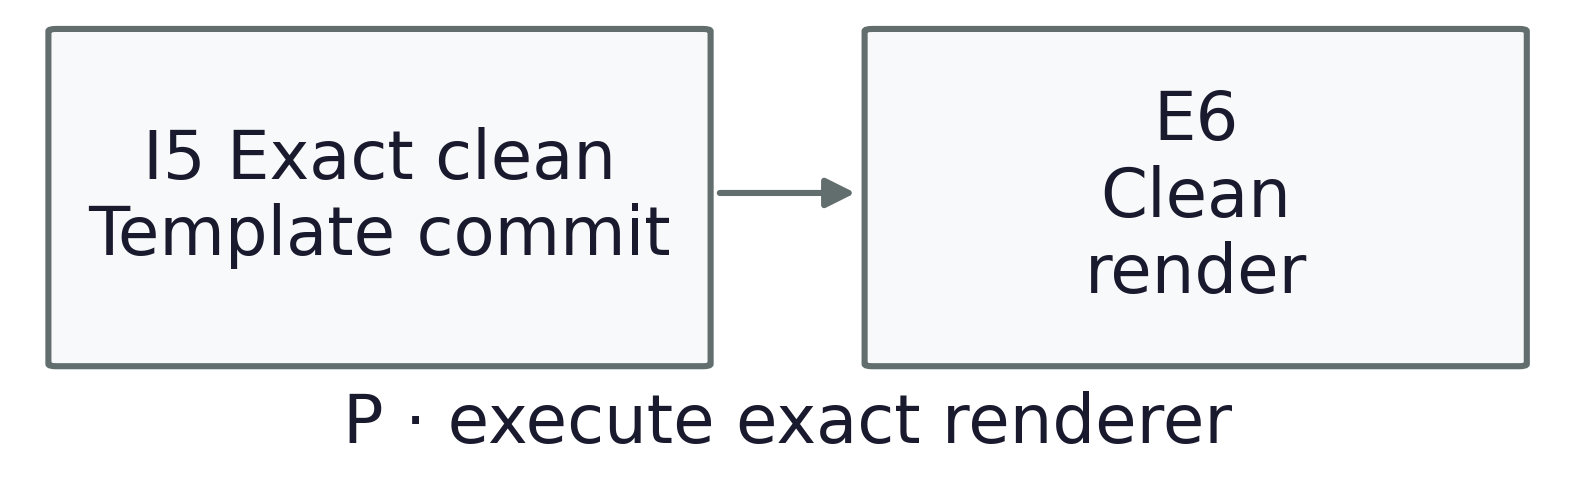
\includegraphics[keepaspectratio,width=0.98\linewidth,height=0.8\textheight,alt={I5  Exact clean Template commit → E6 Clean render: P · execute exact renderer; producer.}]{../figures/source_render_provenance.slide-producer-template-renderer-render.png}
\refstepcounter{figure}\label{fig:source-render-provenance-slide-panel-20}
\end{figure}
\end{frame}

\begin{frame}{Producer order, stale\ldots{} (part 27)}
\begin{figure}
\centering
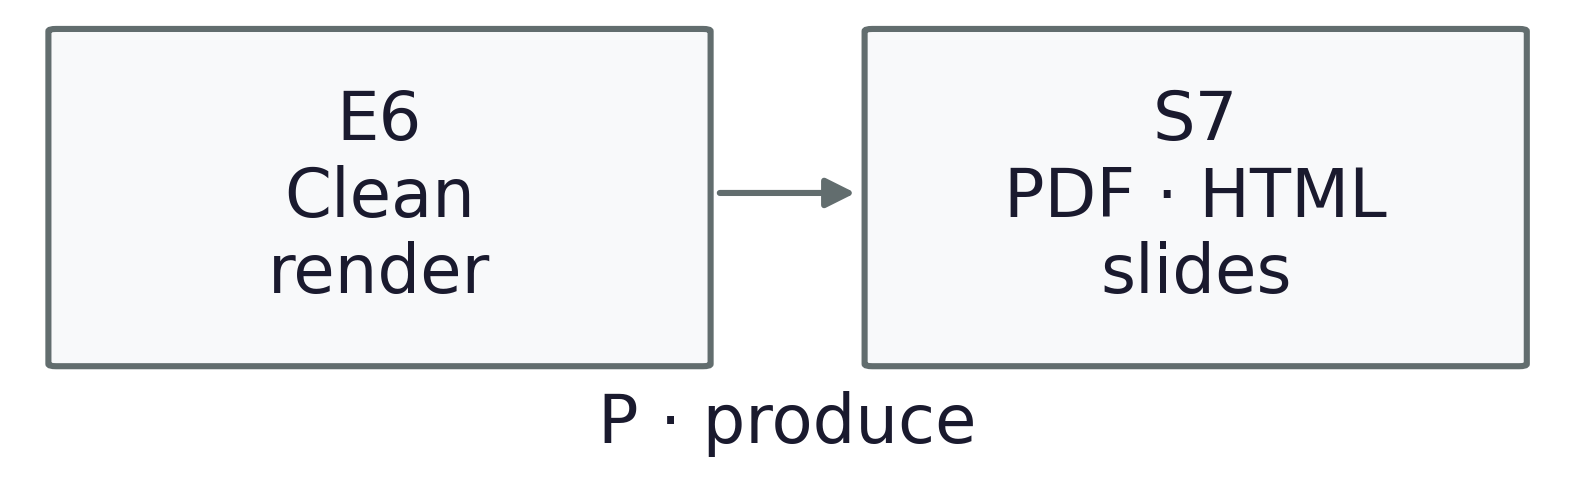
\includegraphics[keepaspectratio,width=0.98\linewidth,height=0.8\textheight,alt={E6 Clean render → S7 PDF · HTML slides: P · produce; producer.}]{../figures/source_render_provenance.slide-producer-render-surfaces.png}
\refstepcounter{figure}\label{fig:source-render-provenance-slide-panel-21}
\end{figure}
\end{frame}

\begin{frame}{Producer order, stale\ldots{} (part 28)}
\begin{figure}
\centering
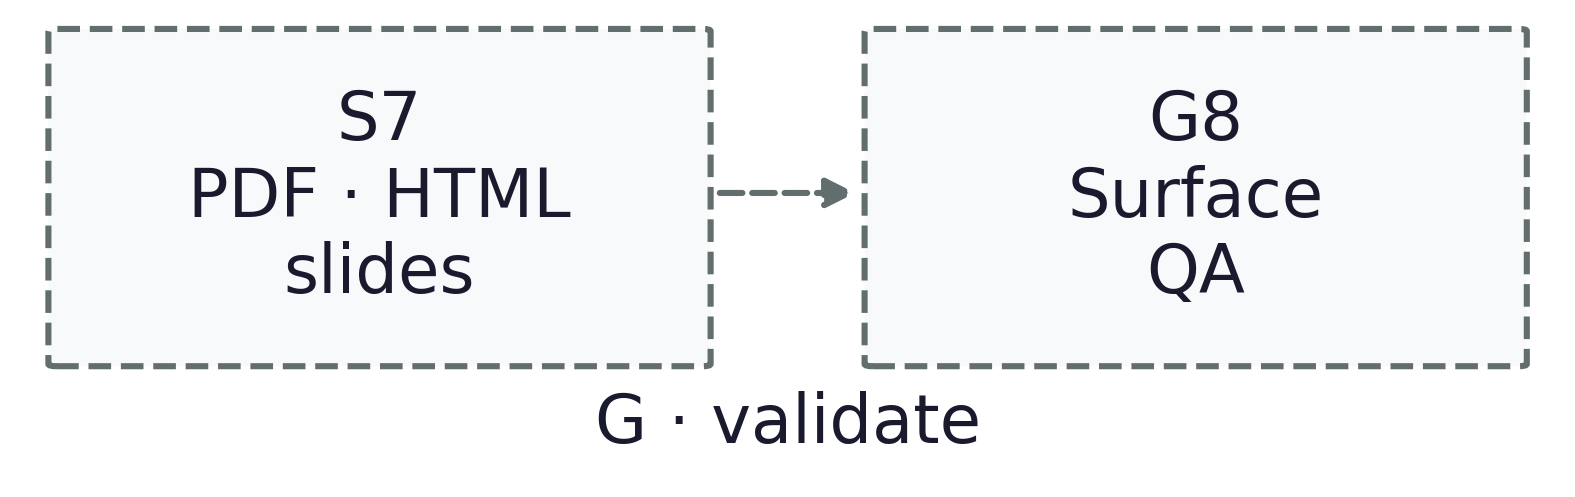
\includegraphics[keepaspectratio,width=0.98\linewidth,height=0.8\textheight,alt={S7 PDF · HTML slides → G8 Surface QA: G · validate; gate.}]{../figures/source_render_provenance.slide-producer-surfaces-surface-validation.png}
\refstepcounter{figure}\label{fig:source-render-provenance-slide-panel-22}
\end{figure}
\end{frame}

\begin{frame}{Producer order, stale\ldots{} (part 29)}
\begin{figure}
\centering
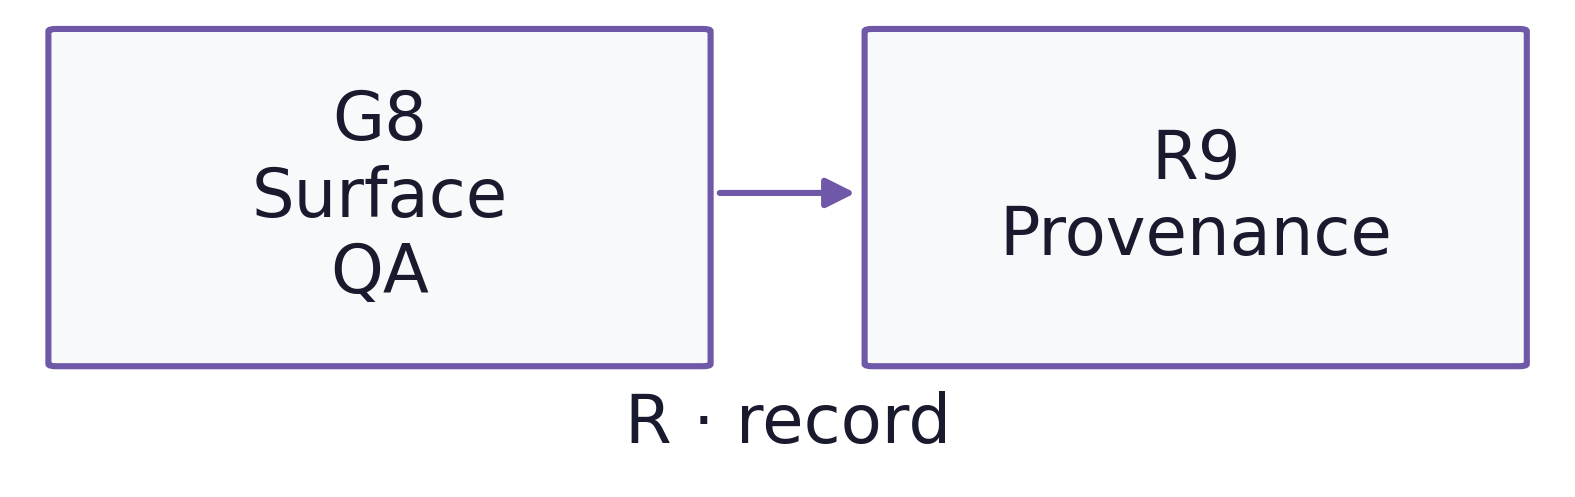
\includegraphics[keepaspectratio,width=0.98\linewidth,height=0.8\textheight,alt={G8 Surface QA → R9 Provenance: R · record; receipt.}]{../figures/source_render_provenance.slide-producer-surface-validation-provenance.png}
\refstepcounter{figure}\label{fig:source-render-provenance-slide-panel-23}
\end{figure}
\end{frame}

\begin{frame}{Producer order, stale\ldots{} (part 30)}
\begin{figure}
\centering
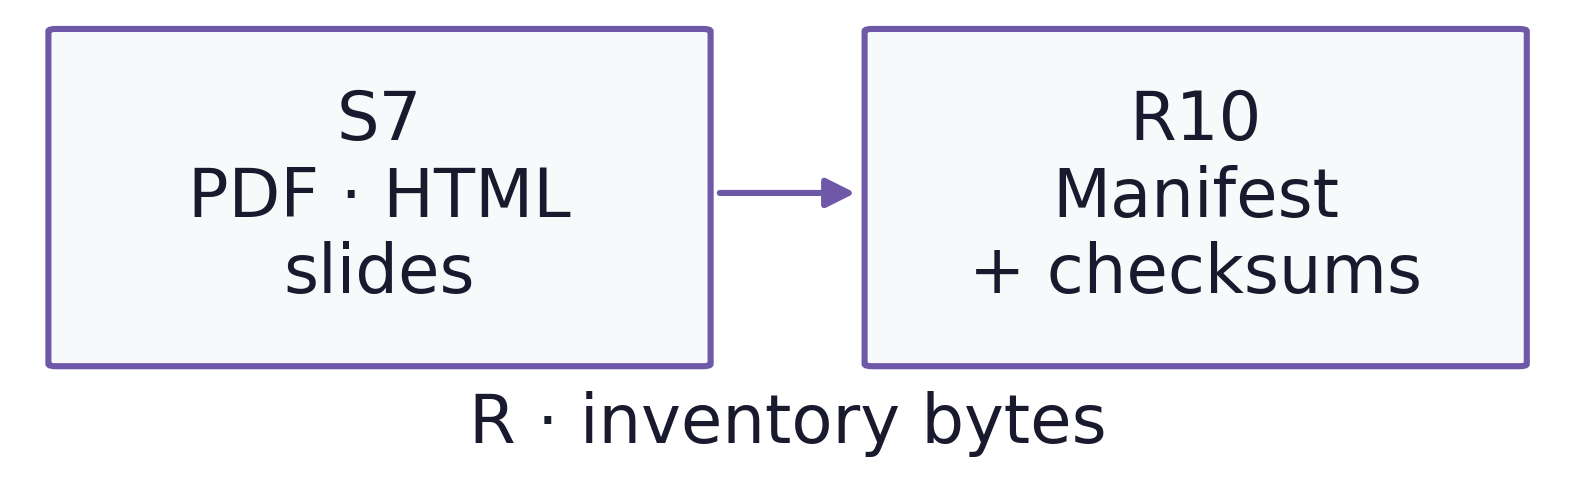
\includegraphics[keepaspectratio,width=0.98\linewidth,height=0.8\textheight,alt={S7 PDF · HTML slides → R10 Manifest + checksums: R · inventory bytes; receipt.}]{../figures/source_render_provenance.slide-producer-surfaces-release-manifest.png}
\refstepcounter{figure}\label{fig:source-render-provenance-slide-panel-24}
\end{figure}
\end{frame}

\begin{frame}{Producer order, stale\ldots{} (part 31)}
\begin{figure}
\centering
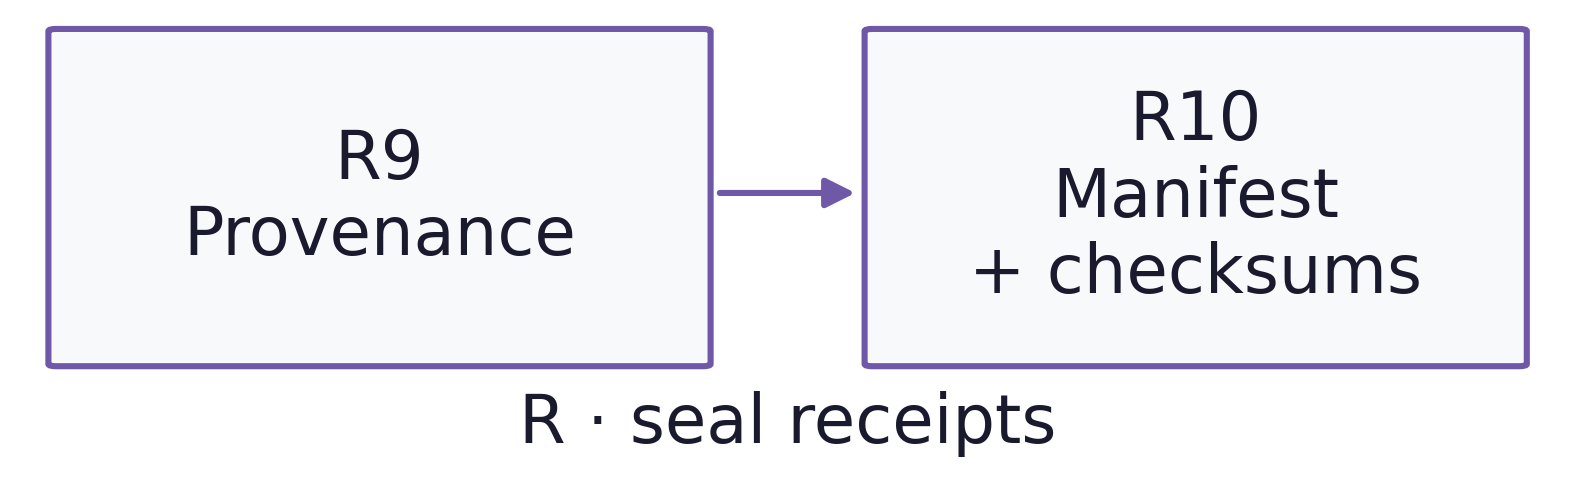
\includegraphics[keepaspectratio,width=0.98\linewidth,height=0.8\textheight,alt={R9 Provenance → R10 Manifest + checksums: R · seal receipts; receipt.}]{../figures/source_render_provenance.slide-producer-provenance-release-manifest.png}
\refstepcounter{figure}\label{fig:source-render-provenance-slide-panel-25}
\end{figure}
\end{frame}

\begin{frame}{Producer order, stale\ldots{} (part 32)}
\begin{figure}
\centering
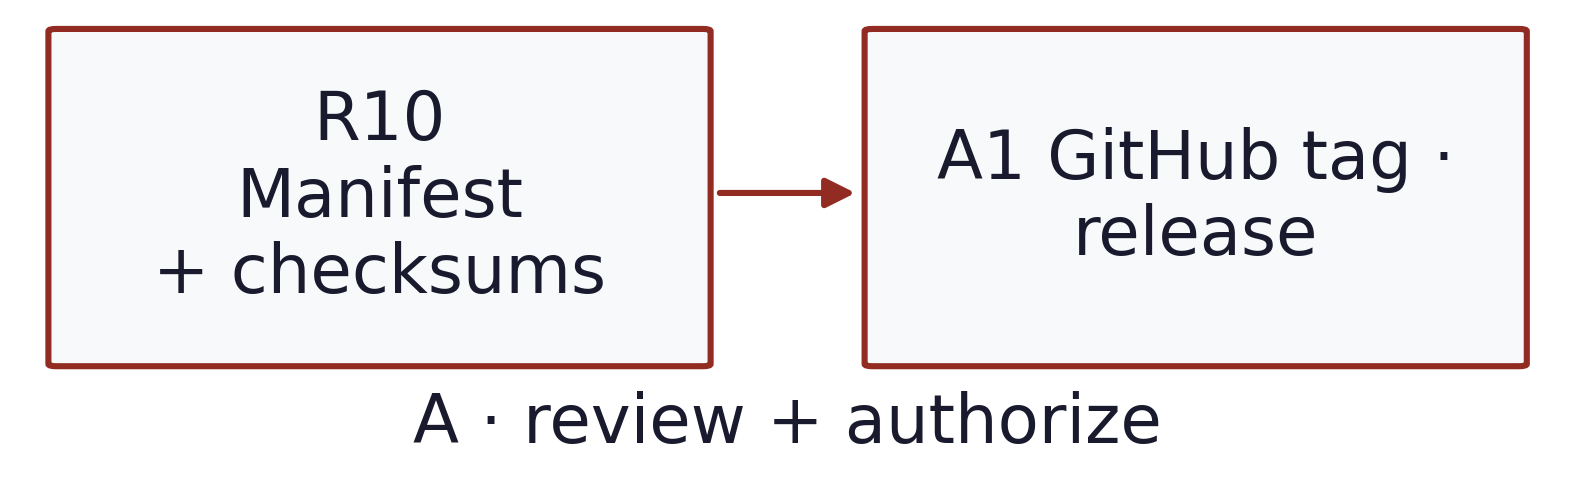
\includegraphics[keepaspectratio,width=0.98\linewidth,height=0.8\textheight,alt={R10 Manifest + checksums → A1  GitHub tag · release: A · review + authorize; authorization.}]{../figures/source_render_provenance.slide-producer-release-manifest-github.png}
\refstepcounter{figure}\label{fig:source-render-provenance-slide-panel-26}
\end{figure}
\end{frame}

\begin{frame}{Producer order, stale\ldots{} (part 33)}
\begin{figure}
\centering
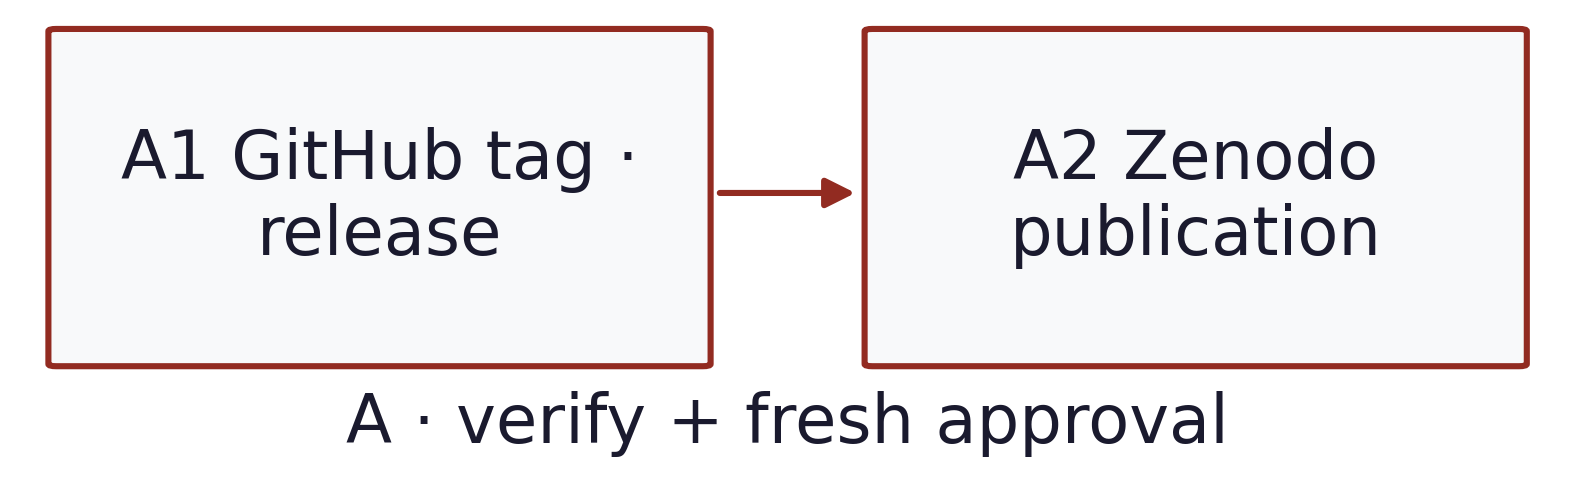
\includegraphics[keepaspectratio,width=0.98\linewidth,height=0.8\textheight,alt={A1  GitHub tag · release → A2  Zenodo publication: A · verify + fresh approval; authorization.}]{../figures/source_render_provenance.slide-producer-github-zenodo.png}
\refstepcounter{figure}\label{fig:source-render-provenance-slide-panel-27}
\end{figure}
\end{frame}

\begin{frame}{Producer order, stale\ldots{} (part 34)}
\begin{figure}
\centering
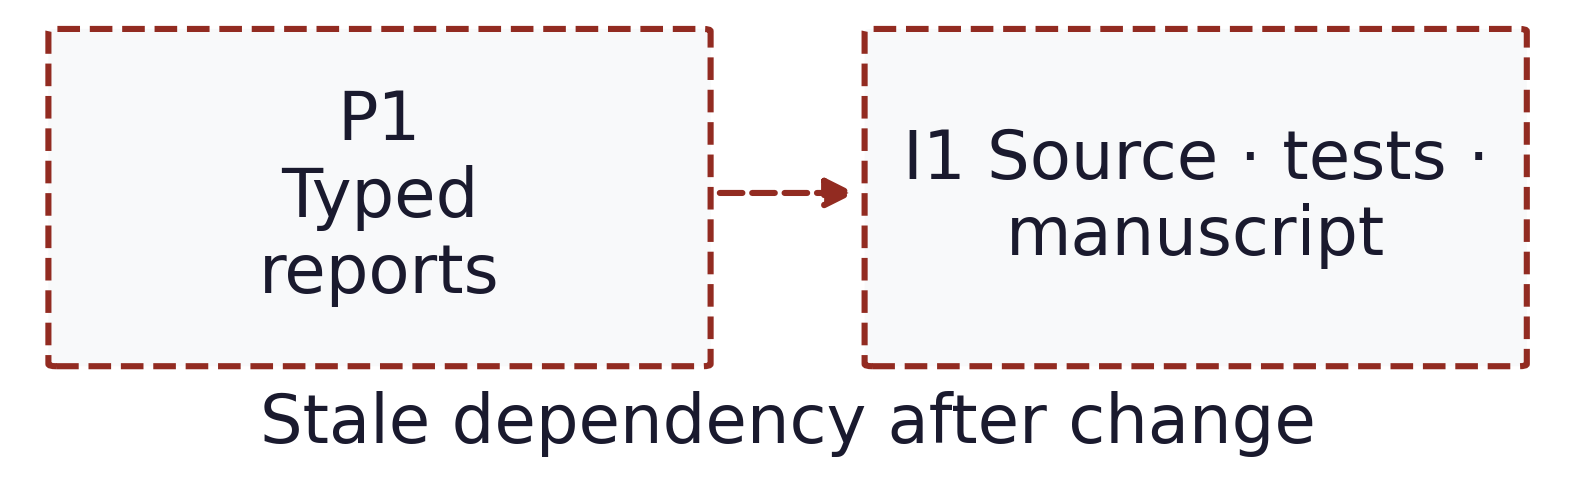
\includegraphics[keepaspectratio,width=0.98\linewidth,height=0.8\textheight,alt={P1 Typed reports → I1  Source · tests · manuscript: Stale dependency after change; invalidation.}]{../figures/source_render_provenance.slide-invalidation-source-reports.png}
\refstepcounter{figure}\label{fig:source-render-provenance-slide-panel-28}
\end{figure}
\end{frame}

\begin{frame}{Producer order, stale\ldots{} (part 35)}
\begin{figure}
\centering
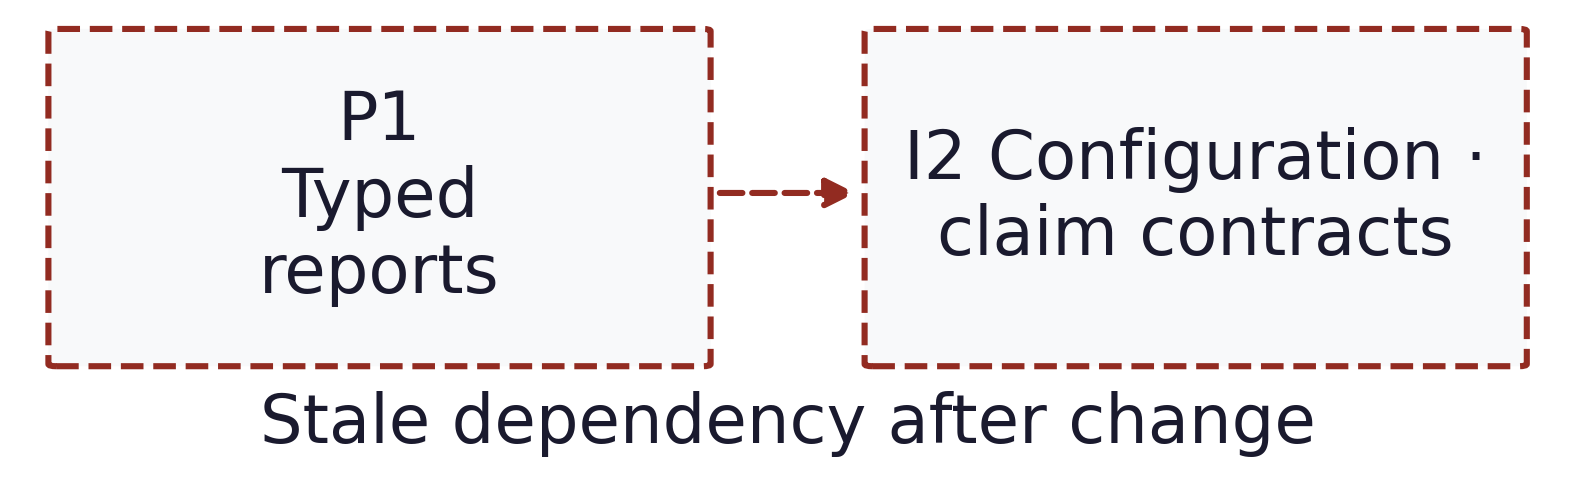
\includegraphics[keepaspectratio,width=0.98\linewidth,height=0.8\textheight,alt={P1 Typed reports → I2  Configuration · claim contracts: Stale dependency after change; invalidation.}]{../figures/source_render_provenance.slide-invalidation-config-reports.png}
\refstepcounter{figure}\label{fig:source-render-provenance-slide-panel-29}
\end{figure}
\end{frame}

\begin{frame}{Producer order, stale\ldots{} (part 36)}
\begin{figure}
\centering
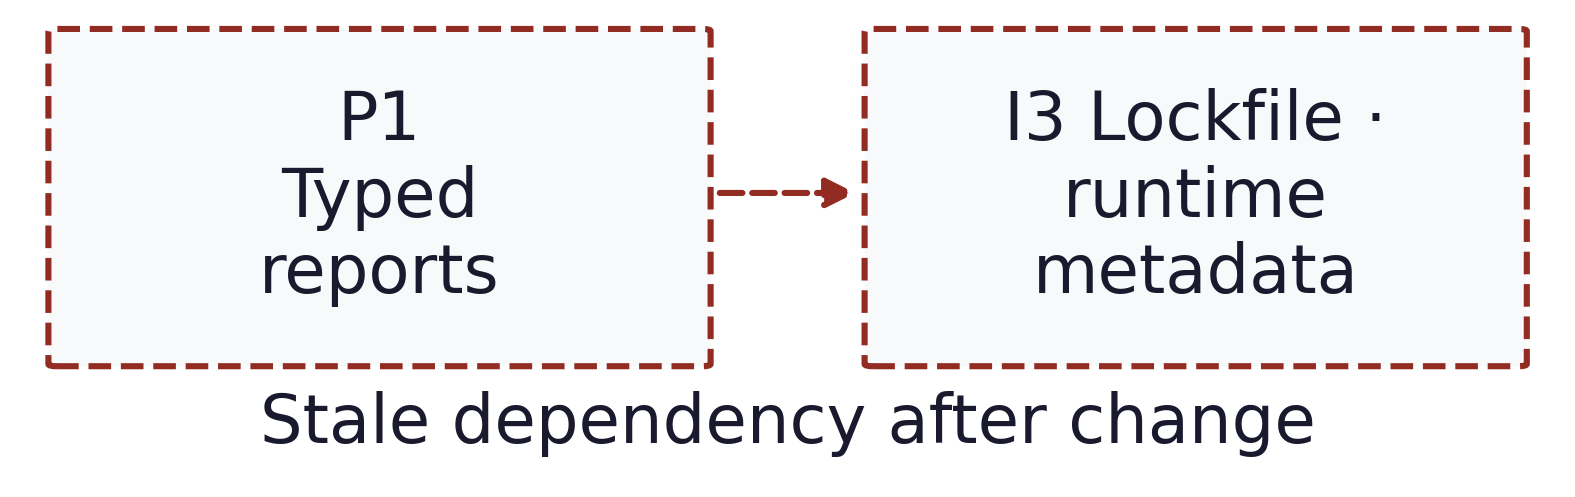
\includegraphics[keepaspectratio,width=0.98\linewidth,height=0.8\textheight,alt={P1 Typed reports → I3  Lockfile · runtime metadata: Stale dependency after change; invalidation.}]{../figures/source_render_provenance.slide-invalidation-lockfile-reports.png}
\refstepcounter{figure}\label{fig:source-render-provenance-slide-panel-30}
\end{figure}
\end{frame}

\begin{frame}{Producer order, stale\ldots{} (part 37)}
\begin{figure}
\centering
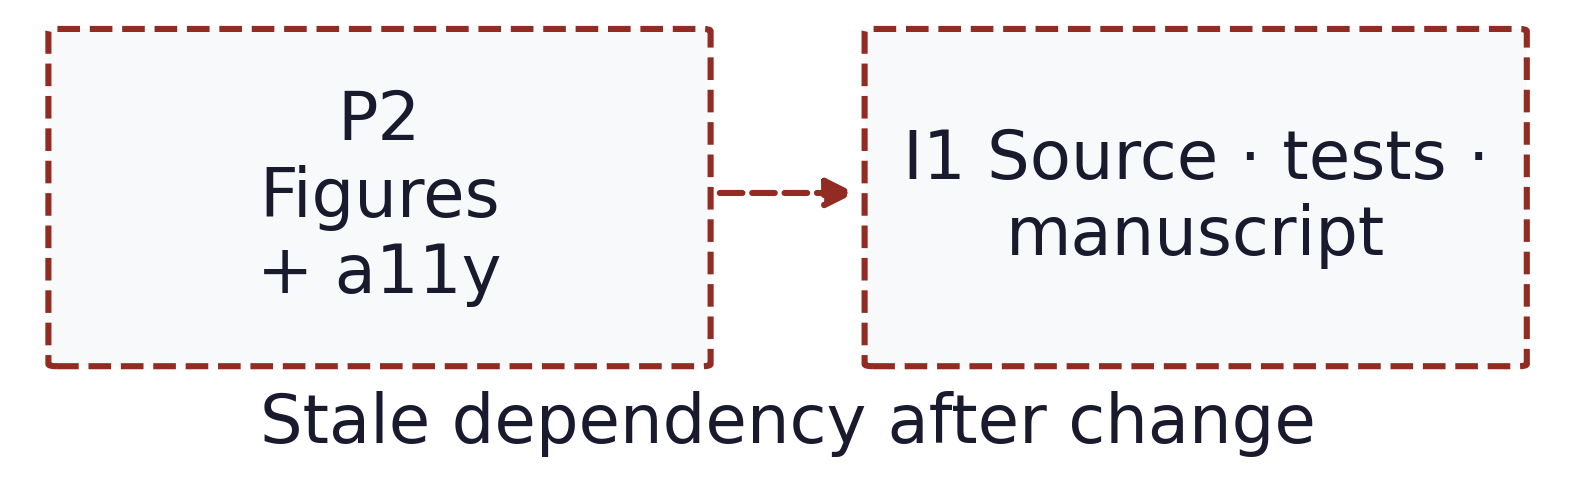
\includegraphics[keepaspectratio,width=0.98\linewidth,height=0.8\textheight,alt={P2 Figures + a11y → I1  Source · tests · manuscript: Stale dependency after change; invalidation.}]{../figures/source_render_provenance.slide-invalidation-source-figures.png}
\refstepcounter{figure}\label{fig:source-render-provenance-slide-panel-31}
\end{figure}
\end{frame}

\begin{frame}{Producer order, stale\ldots{} (part 38)}
\begin{figure}
\centering
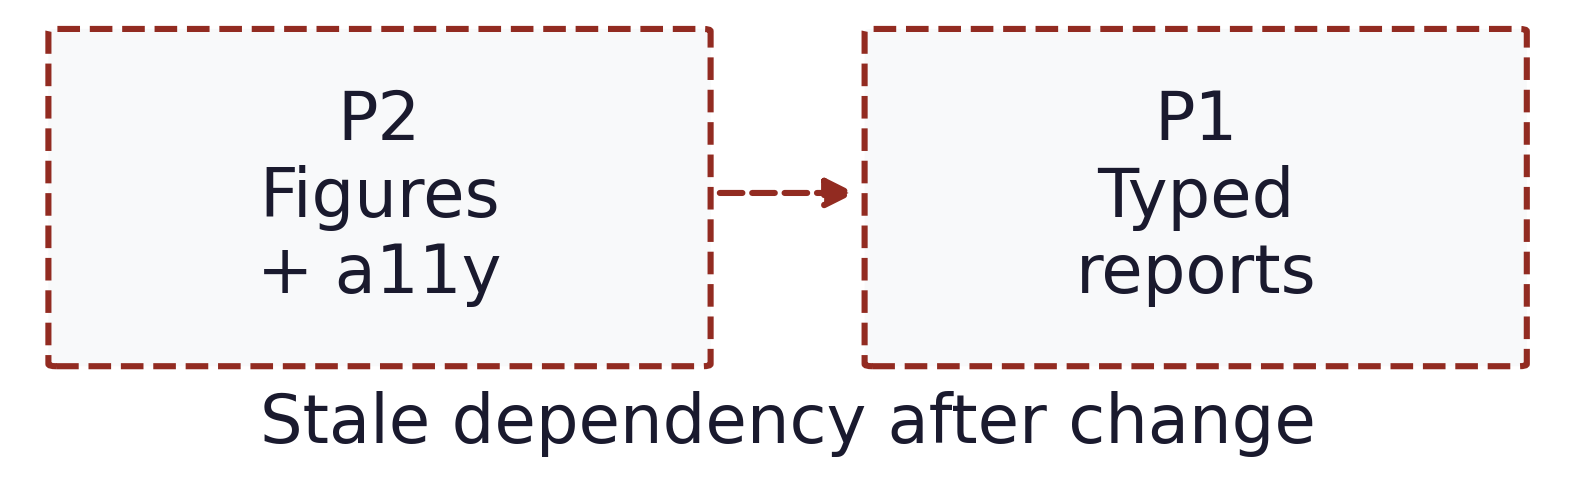
\includegraphics[keepaspectratio,width=0.98\linewidth,height=0.8\textheight,alt={P2 Figures + a11y → P1 Typed reports: Stale dependency after change; invalidation.}]{../figures/source_render_provenance.slide-invalidation-reports-figures.png}
\refstepcounter{figure}\label{fig:source-render-provenance-slide-panel-32}
\end{figure}
\end{frame}

\begin{frame}{Producer order, stale\ldots{} (part 39)}
\begin{figure}
\centering
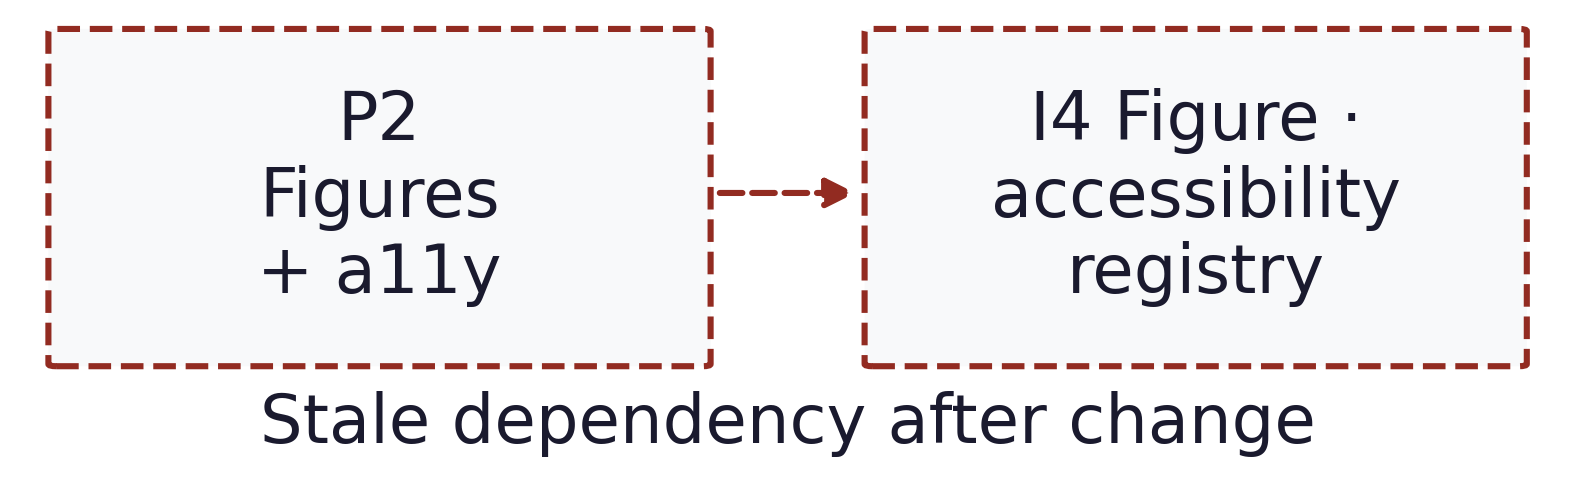
\includegraphics[keepaspectratio,width=0.98\linewidth,height=0.8\textheight,alt={P2 Figures + a11y → I4  Figure · accessibility registry: Stale dependency after change; invalidation.}]{../figures/source_render_provenance.slide-invalidation-registry-figures.png}
\refstepcounter{figure}\label{fig:source-render-provenance-slide-panel-33}
\end{figure}
\end{frame}

\begin{frame}{Producer order, stale\ldots{} (part 40)}
\begin{figure}
\centering
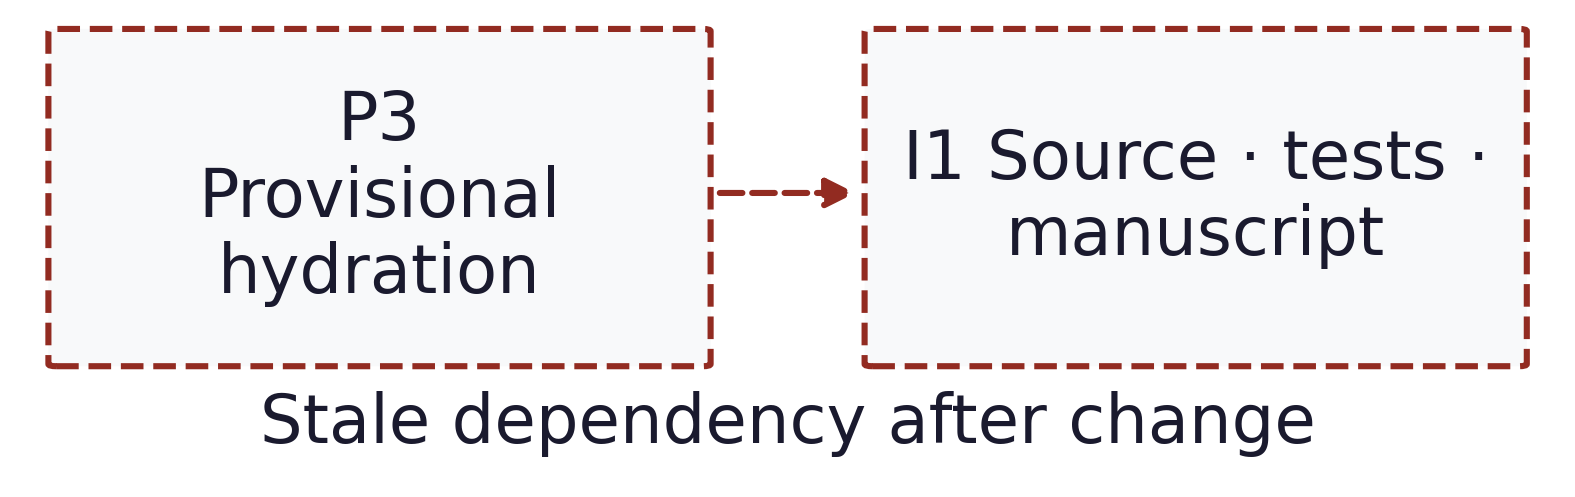
\includegraphics[keepaspectratio,width=0.98\linewidth,height=0.8\textheight,alt={P3 Provisional hydration → I1  Source · tests · manuscript: Stale dependency after change; invalidation.}]{../figures/source_render_provenance.slide-invalidation-source-provisional.png}
\refstepcounter{figure}\label{fig:source-render-provenance-slide-panel-34}
\end{figure}
\end{frame}

\begin{frame}{Producer order, stale\ldots{} (part 41)}
\begin{figure}
\centering
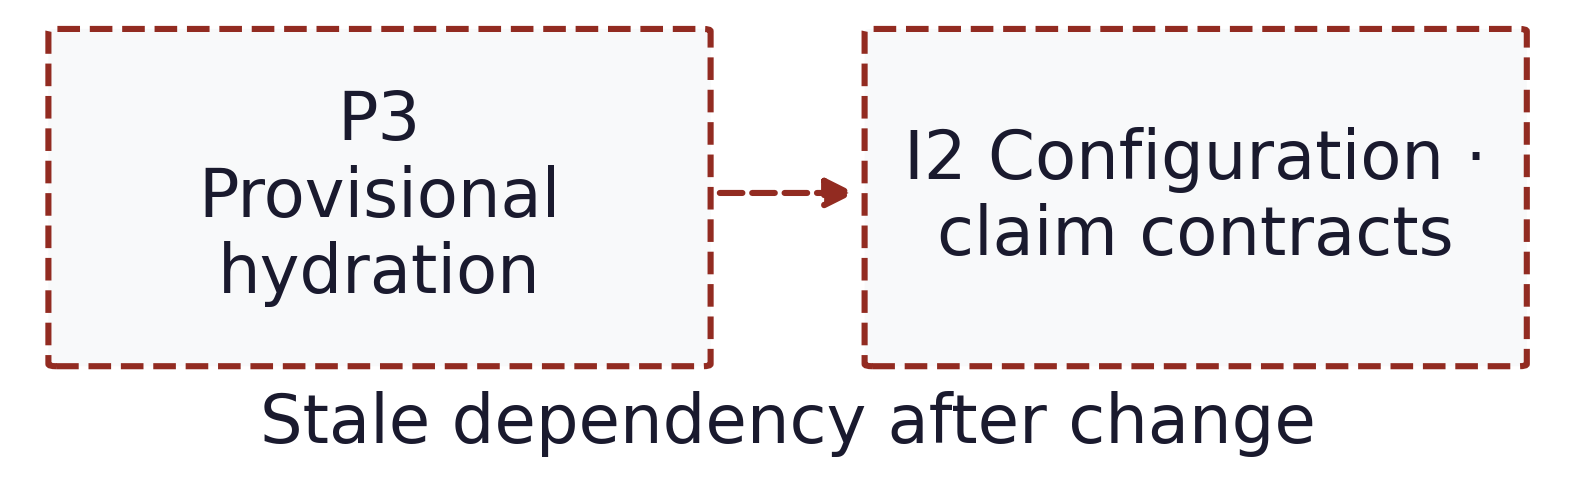
\includegraphics[keepaspectratio,width=0.98\linewidth,height=0.8\textheight,alt={P3 Provisional hydration → I2  Configuration · claim contracts: Stale dependency after change; invalidation.}]{../figures/source_render_provenance.slide-invalidation-config-provisional.png}
\refstepcounter{figure}\label{fig:source-render-provenance-slide-panel-35}
\end{figure}
\end{frame}

\begin{frame}{Producer order, stale\ldots{} (part 42)}
\begin{figure}
\centering
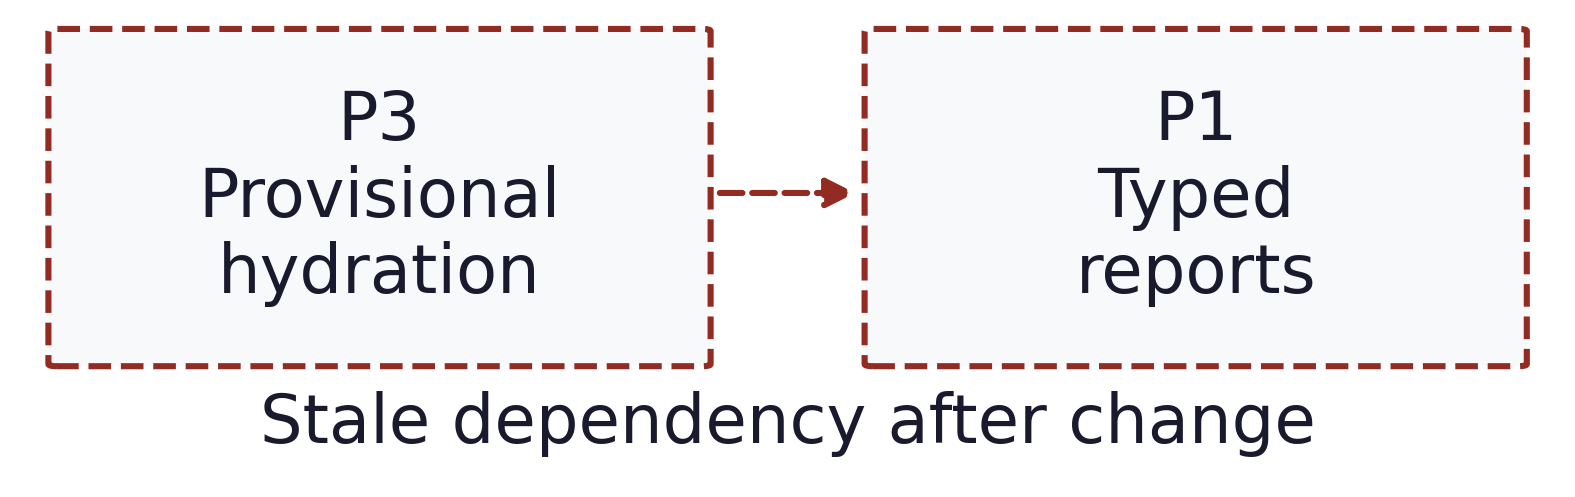
\includegraphics[keepaspectratio,width=0.98\linewidth,height=0.8\textheight,alt={P3 Provisional hydration → P1 Typed reports: Stale dependency after change; invalidation.}]{../figures/source_render_provenance.slide-invalidation-reports-provisional.png}
\refstepcounter{figure}\label{fig:source-render-provenance-slide-panel-36}
\end{figure}
\end{frame}

\begin{frame}{Producer order, stale\ldots{} (part 43)}
\begin{figure}
\centering
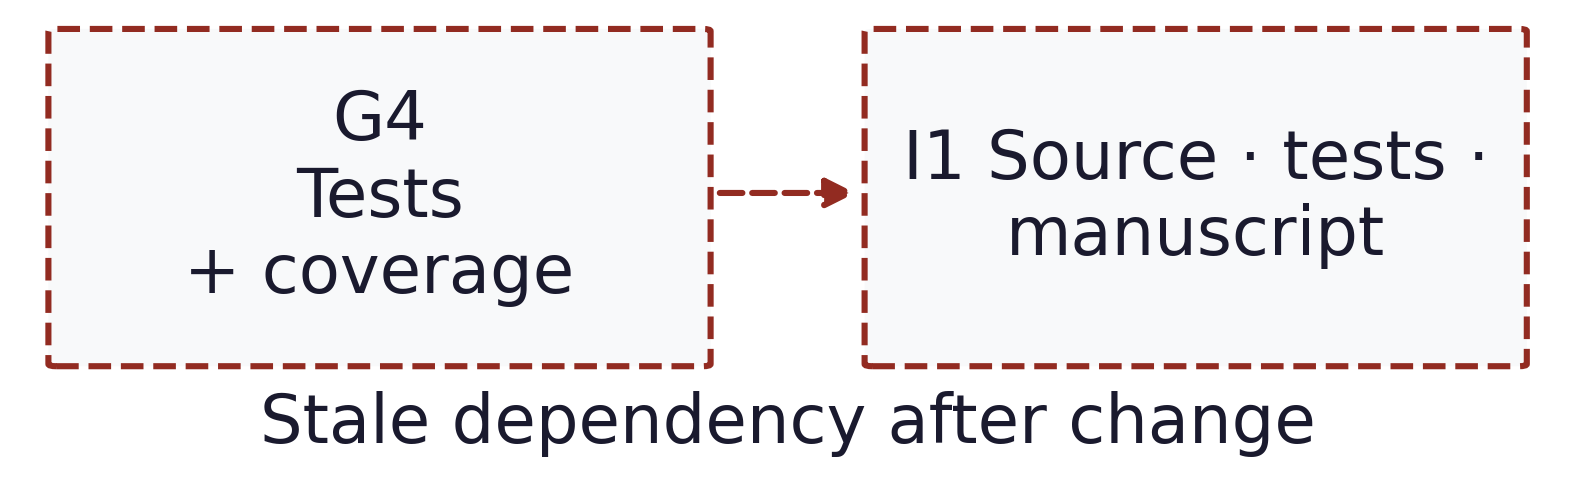
\includegraphics[keepaspectratio,width=0.98\linewidth,height=0.8\textheight,alt={G4 Tests + coverage → I1  Source · tests · manuscript: Stale dependency after change; invalidation.}]{../figures/source_render_provenance.slide-invalidation-source-coverage.png}
\refstepcounter{figure}\label{fig:source-render-provenance-slide-panel-37}
\end{figure}
\end{frame}

\begin{frame}{Producer order, stale\ldots{} (part 44)}
\begin{figure}
\centering
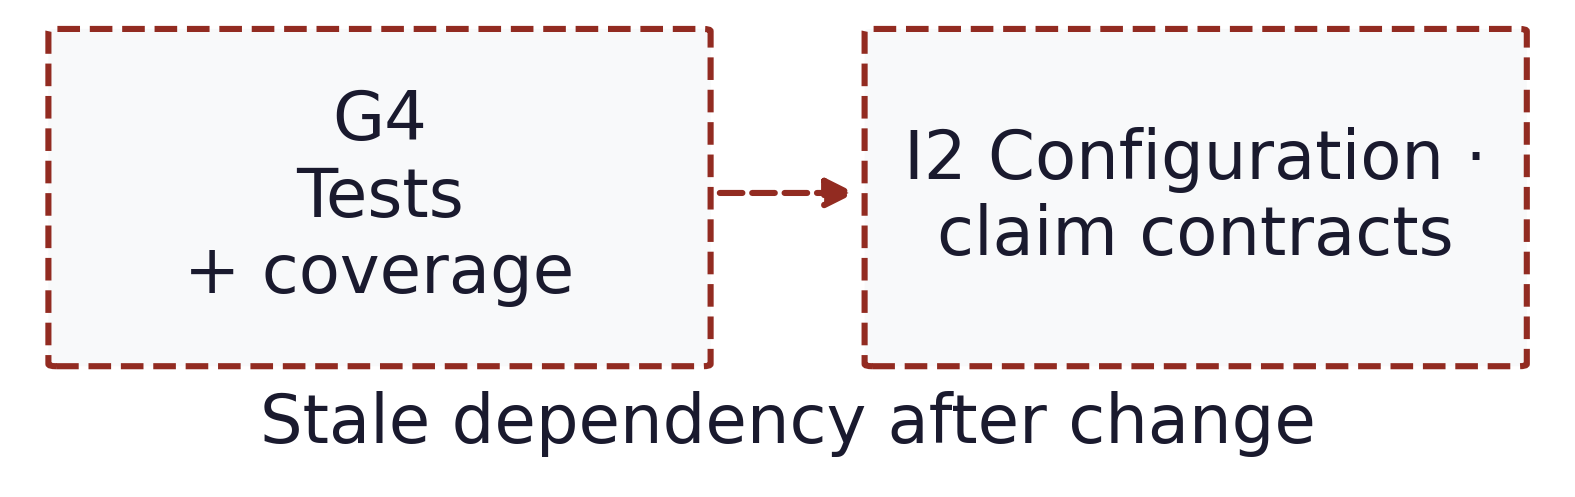
\includegraphics[keepaspectratio,width=0.98\linewidth,height=0.8\textheight,alt={G4 Tests + coverage → I2  Configuration · claim contracts: Stale dependency after change; invalidation.}]{../figures/source_render_provenance.slide-invalidation-config-coverage.png}
\refstepcounter{figure}\label{fig:source-render-provenance-slide-panel-38}
\end{figure}
\end{frame}

\begin{frame}{Producer order, stale\ldots{} (part 45)}
\begin{figure}
\centering
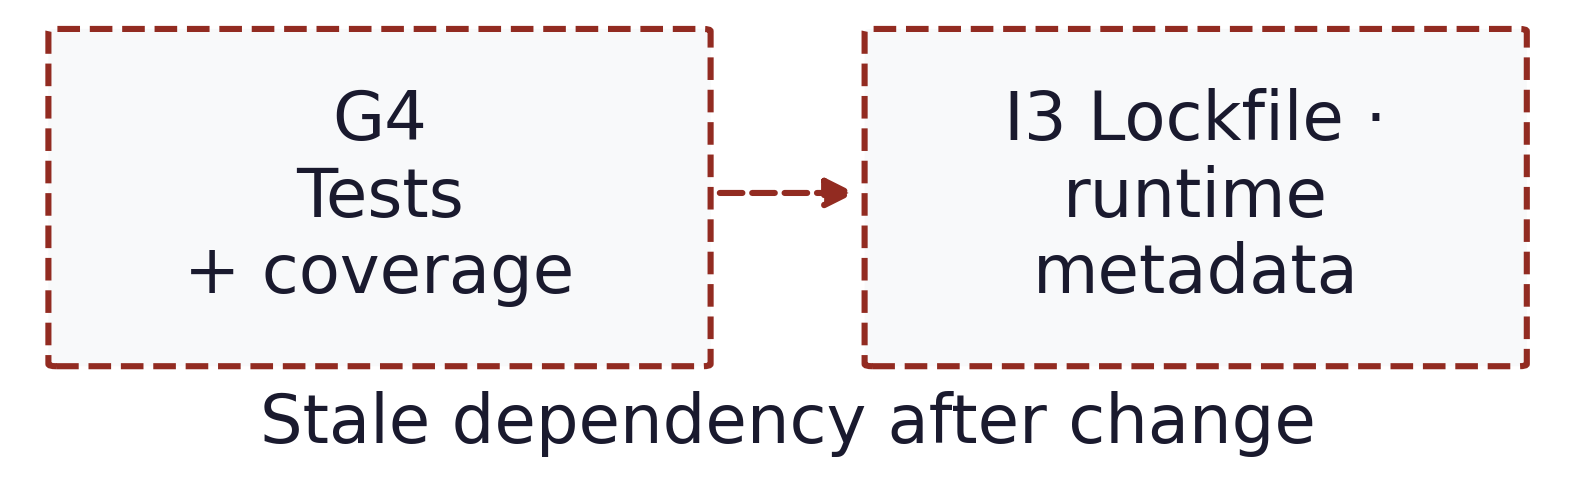
\includegraphics[keepaspectratio,width=0.98\linewidth,height=0.8\textheight,alt={G4 Tests + coverage → I3  Lockfile · runtime metadata: Stale dependency after change; invalidation.}]{../figures/source_render_provenance.slide-invalidation-lockfile-coverage.png}
\refstepcounter{figure}\label{fig:source-render-provenance-slide-panel-39}
\end{figure}
\end{frame}

\begin{frame}{Producer order, stale\ldots{} (part 46)}
\begin{figure}
\centering
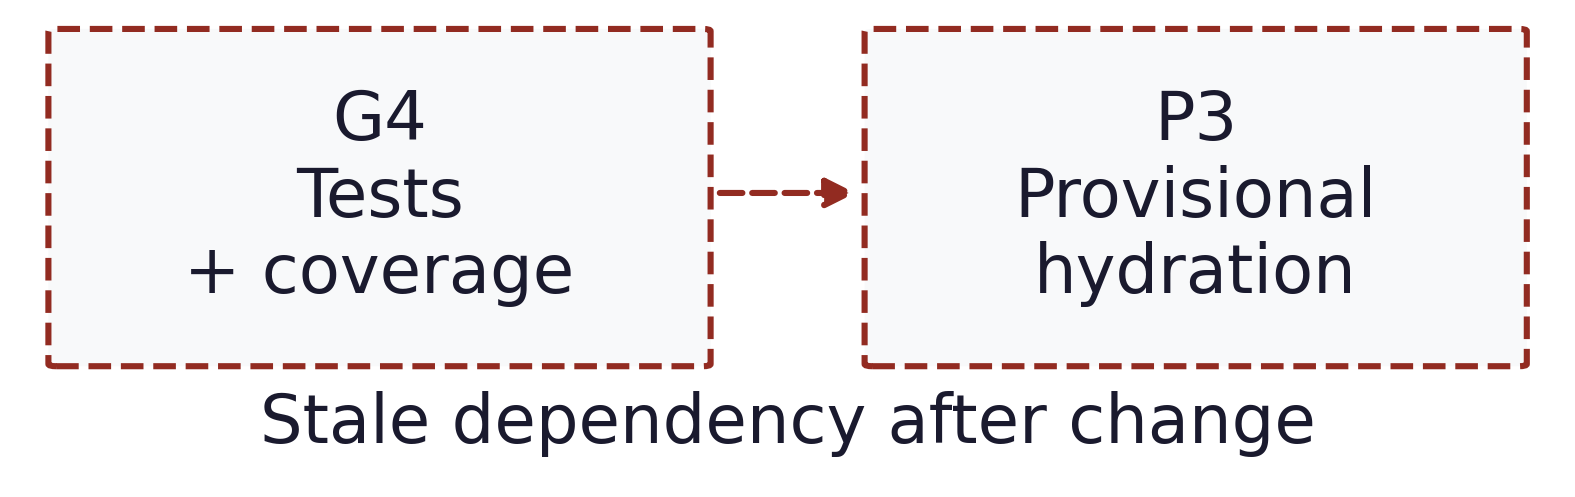
\includegraphics[keepaspectratio,width=0.98\linewidth,height=0.8\textheight,alt={G4 Tests + coverage → P3 Provisional hydration: Stale dependency after change; invalidation.}]{../figures/source_render_provenance.slide-invalidation-provisional-coverage.png}
\refstepcounter{figure}\label{fig:source-render-provenance-slide-panel-40}
\end{figure}
\end{frame}

\begin{frame}{Producer order, stale\ldots{} (part 47)}
\begin{figure}
\centering
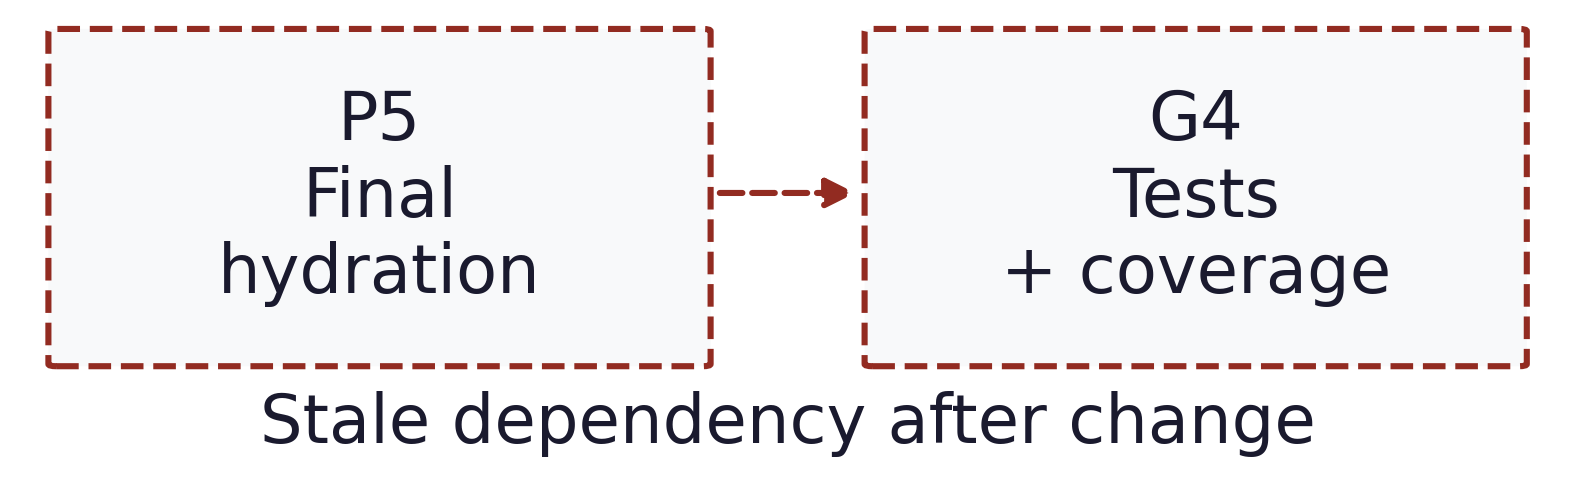
\includegraphics[keepaspectratio,width=0.98\linewidth,height=0.8\textheight,alt={P5 Final hydration → G4 Tests + coverage: Stale dependency after change; invalidation.}]{../figures/source_render_provenance.slide-invalidation-coverage-final-hydration.png}
\refstepcounter{figure}\label{fig:source-render-provenance-slide-panel-41}
\end{figure}
\end{frame}

\begin{frame}{Producer order, stale\ldots{} (part 48)}
\begin{figure}
\centering
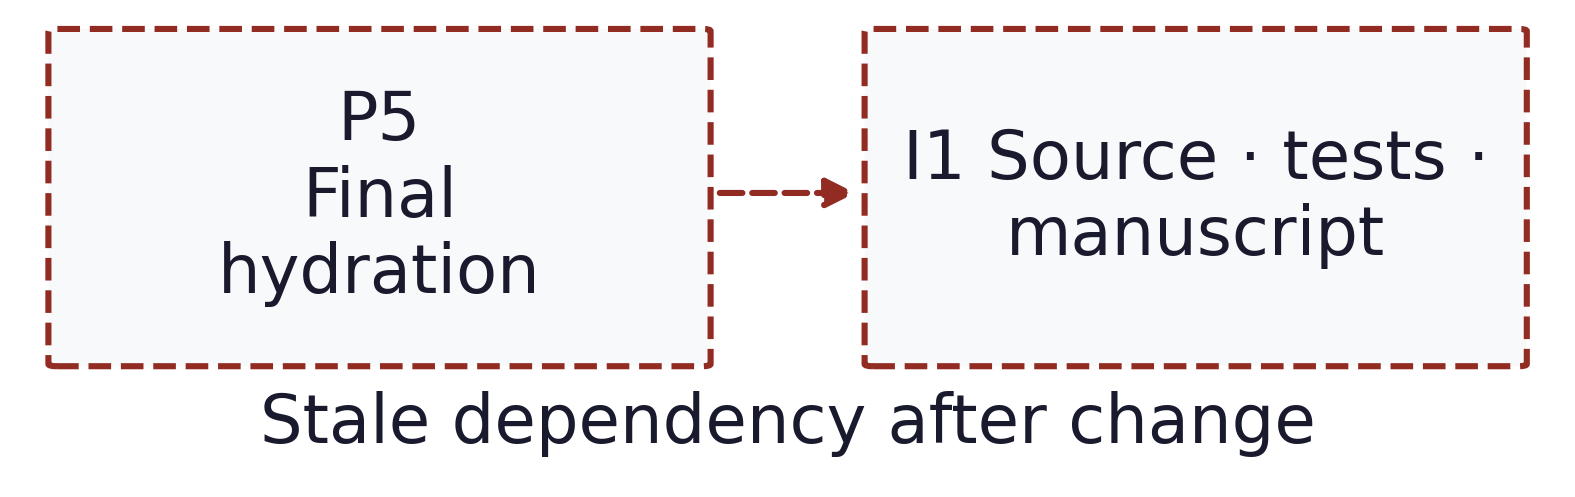
\includegraphics[keepaspectratio,width=0.98\linewidth,height=0.8\textheight,alt={P5 Final hydration → I1  Source · tests · manuscript: Stale dependency after change; invalidation.}]{../figures/source_render_provenance.slide-invalidation-source-final-hydration.png}
\refstepcounter{figure}\label{fig:source-render-provenance-slide-panel-42}
\end{figure}
\end{frame}

\begin{frame}{Producer order, stale\ldots{} (part 49)}
\begin{figure}
\centering
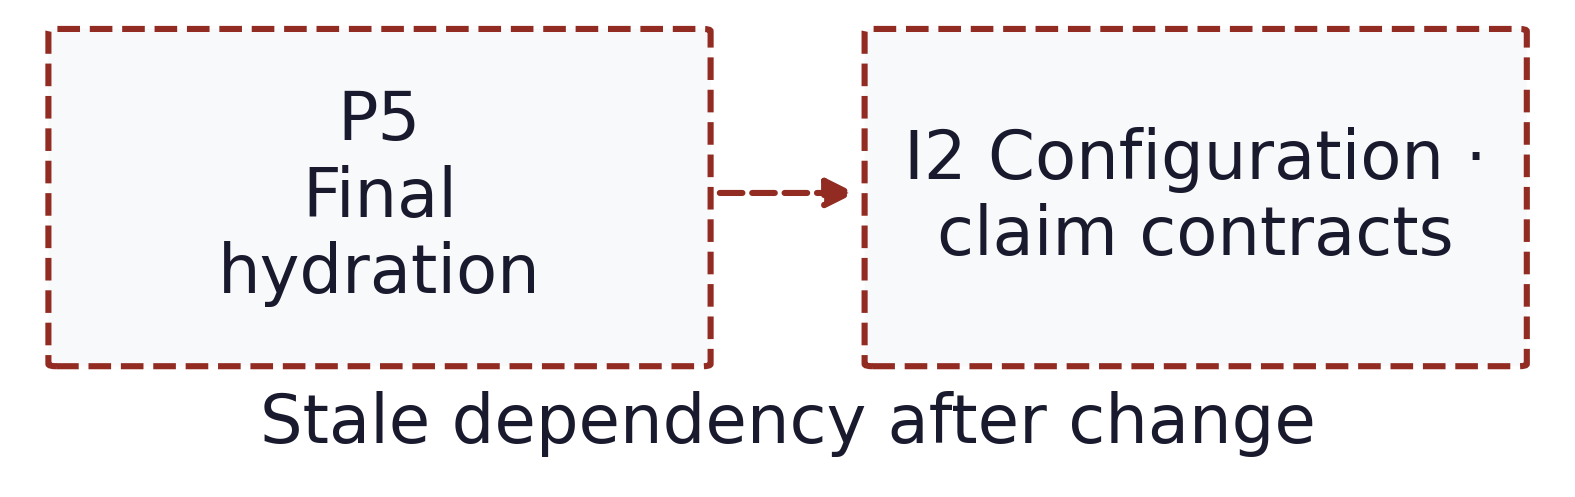
\includegraphics[keepaspectratio,width=0.98\linewidth,height=0.8\textheight,alt={P5 Final hydration → I2  Configuration · claim contracts: Stale dependency after change; invalidation.}]{../figures/source_render_provenance.slide-invalidation-config-final-hydration.png}
\refstepcounter{figure}\label{fig:source-render-provenance-slide-panel-43}
\end{figure}
\end{frame}

\begin{frame}{Producer order, stale\ldots{} (part 50)}
\begin{figure}
\centering
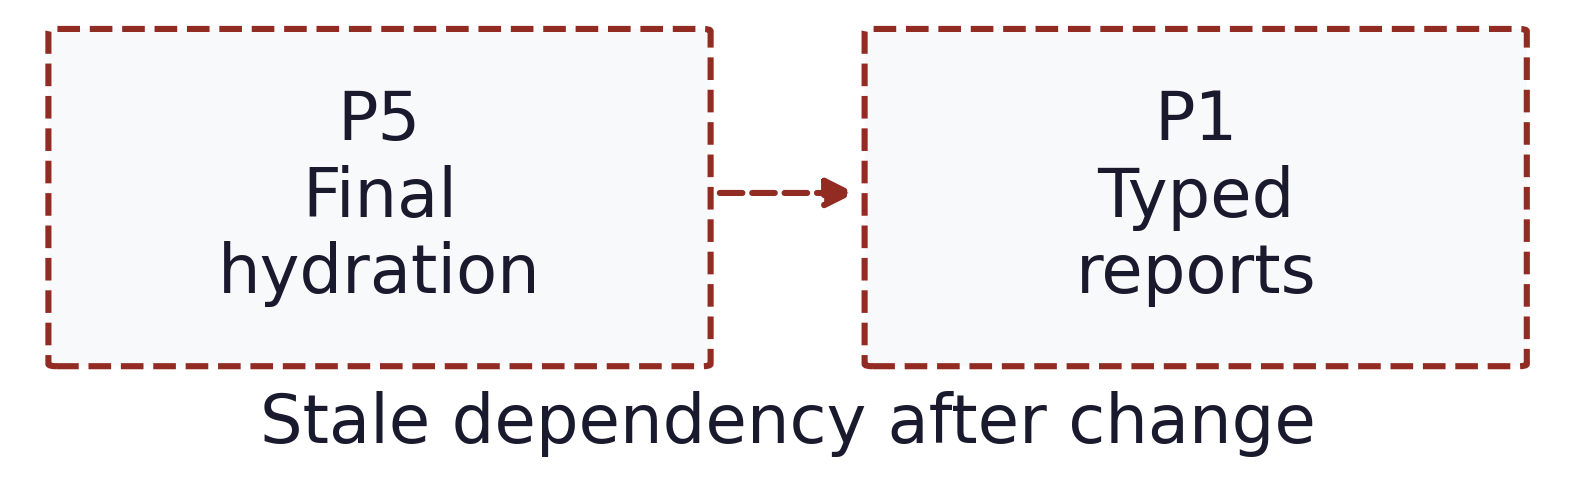
\includegraphics[keepaspectratio,width=0.98\linewidth,height=0.8\textheight,alt={P5 Final hydration → P1 Typed reports: Stale dependency after change; invalidation.}]{../figures/source_render_provenance.slide-invalidation-reports-final-hydration.png}
\refstepcounter{figure}\label{fig:source-render-provenance-slide-panel-44}
\end{figure}
\end{frame}

\begin{frame}{Producer order, stale\ldots{} (part 51)}
\begin{figure}
\centering
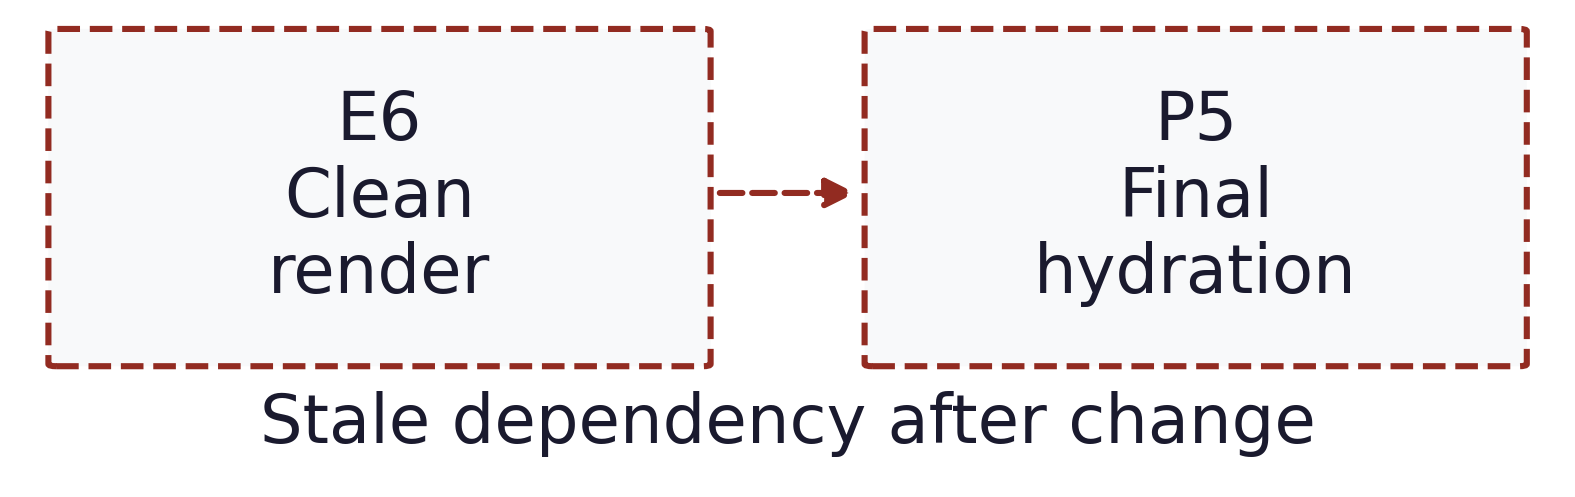
\includegraphics[keepaspectratio,width=0.98\linewidth,height=0.8\textheight,alt={E6 Clean render → P5 Final hydration: Stale dependency after change; invalidation.}]{../figures/source_render_provenance.slide-invalidation-final-hydration-render.png}
\refstepcounter{figure}\label{fig:source-render-provenance-slide-panel-45}
\end{figure}
\end{frame}

\begin{frame}{Producer order, stale\ldots{} (part 52)}
\begin{figure}
\centering
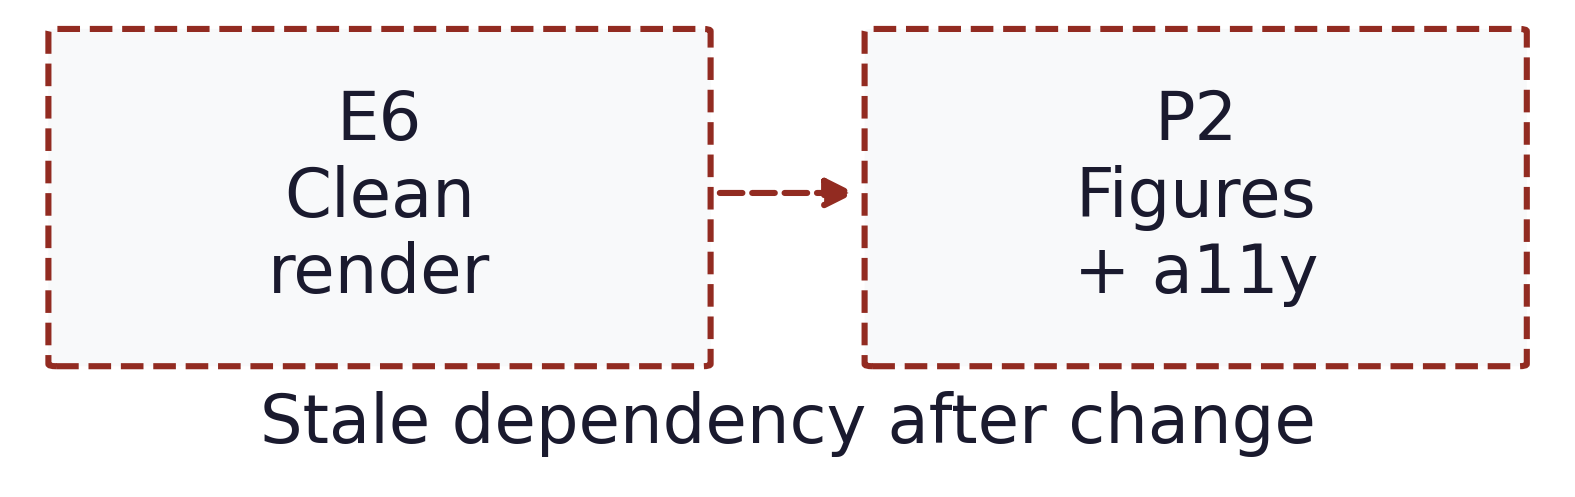
\includegraphics[keepaspectratio,width=0.98\linewidth,height=0.8\textheight,alt={E6 Clean render → P2 Figures + a11y: Stale dependency after change; invalidation.}]{../figures/source_render_provenance.slide-invalidation-figures-render.png}
\refstepcounter{figure}\label{fig:source-render-provenance-slide-panel-46}
\end{figure}
\end{frame}

\begin{frame}{Producer order, stale\ldots{} (part 53)}
\begin{figure}
\centering
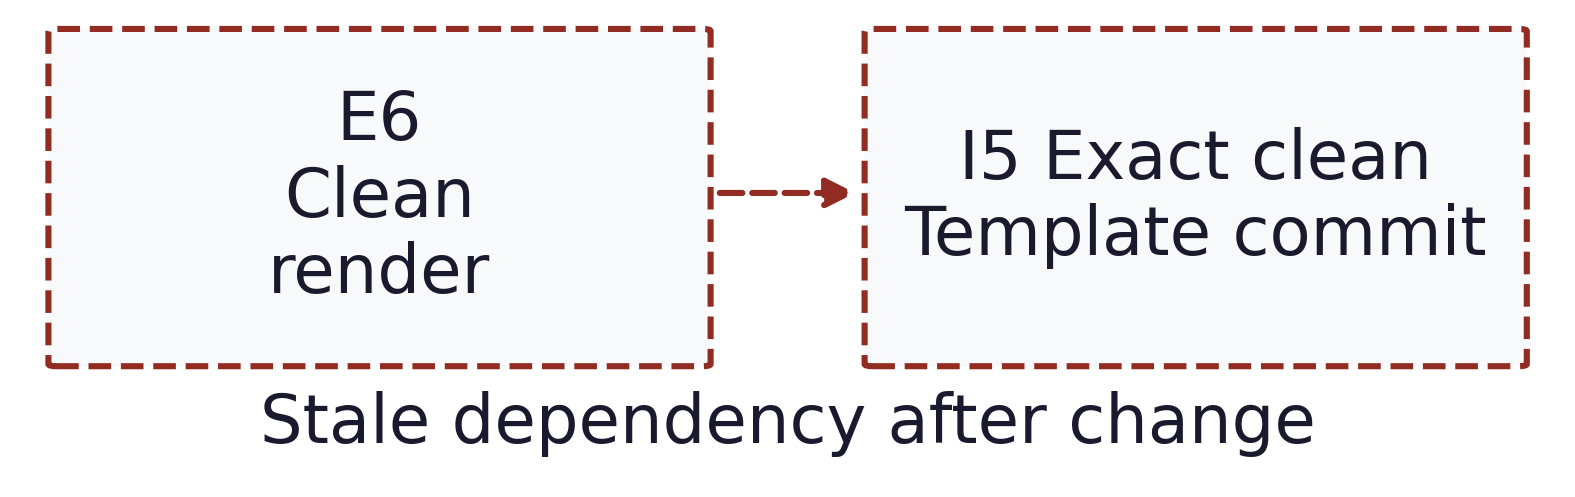
\includegraphics[keepaspectratio,width=0.98\linewidth,height=0.8\textheight,alt={E6 Clean render → I5  Exact clean Template commit: Stale dependency after change; invalidation.}]{../figures/source_render_provenance.slide-invalidation-template-renderer-render.png}
\refstepcounter{figure}\label{fig:source-render-provenance-slide-panel-47}
\end{figure}
\end{frame}

\begin{frame}{Producer order, stale\ldots{} (part 54)}
\begin{figure}
\centering
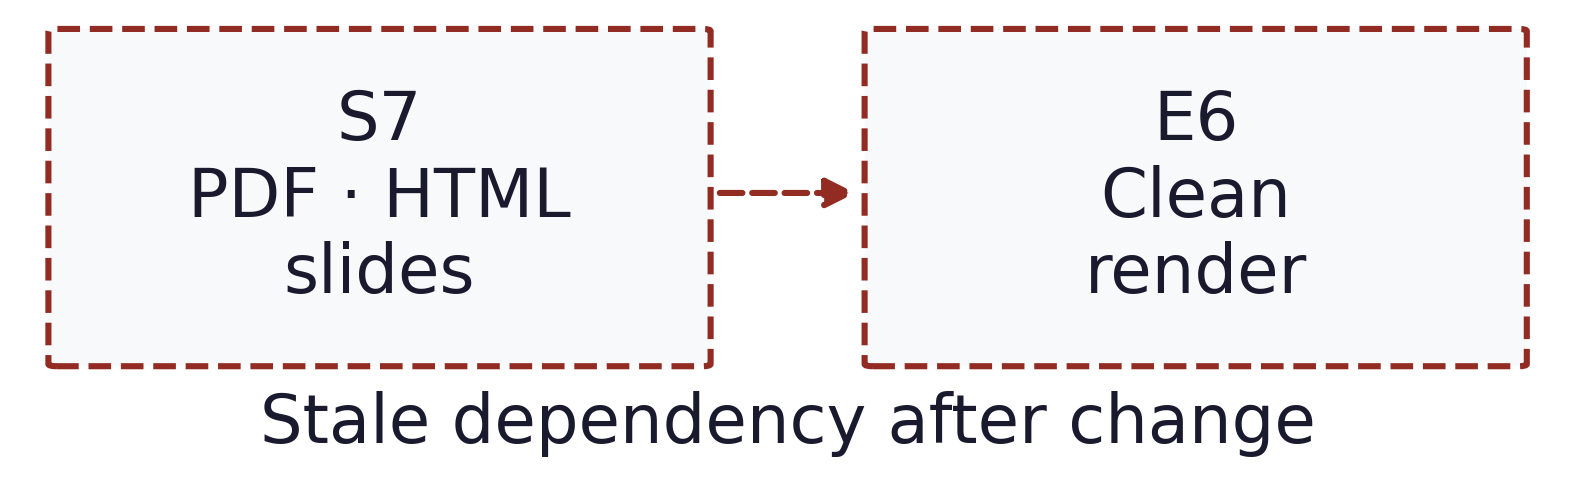
\includegraphics[keepaspectratio,width=0.98\linewidth,height=0.8\textheight,alt={S7 PDF · HTML slides → E6 Clean render: Stale dependency after change; invalidation.}]{../figures/source_render_provenance.slide-invalidation-render-surfaces.png}
\refstepcounter{figure}\label{fig:source-render-provenance-slide-panel-48}
\end{figure}
\end{frame}

\begin{frame}{Producer order, stale\ldots{} (part 55)}
\begin{figure}
\centering
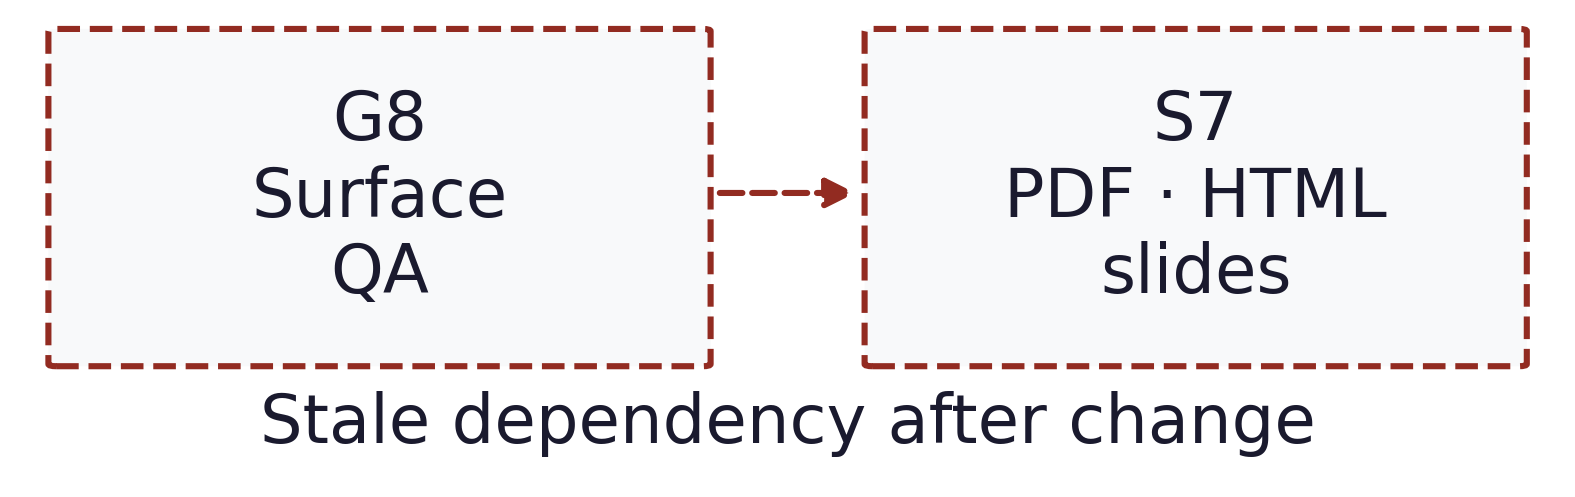
\includegraphics[keepaspectratio,width=0.98\linewidth,height=0.8\textheight,alt={G8 Surface QA → S7 PDF · HTML slides: Stale dependency after change; invalidation.}]{../figures/source_render_provenance.slide-invalidation-surfaces-surface-validation.png}
\refstepcounter{figure}\label{fig:source-render-provenance-slide-panel-49}
\end{figure}
\end{frame}

\begin{frame}{Producer order, stale\ldots{} (part 56)}
\begin{figure}
\centering
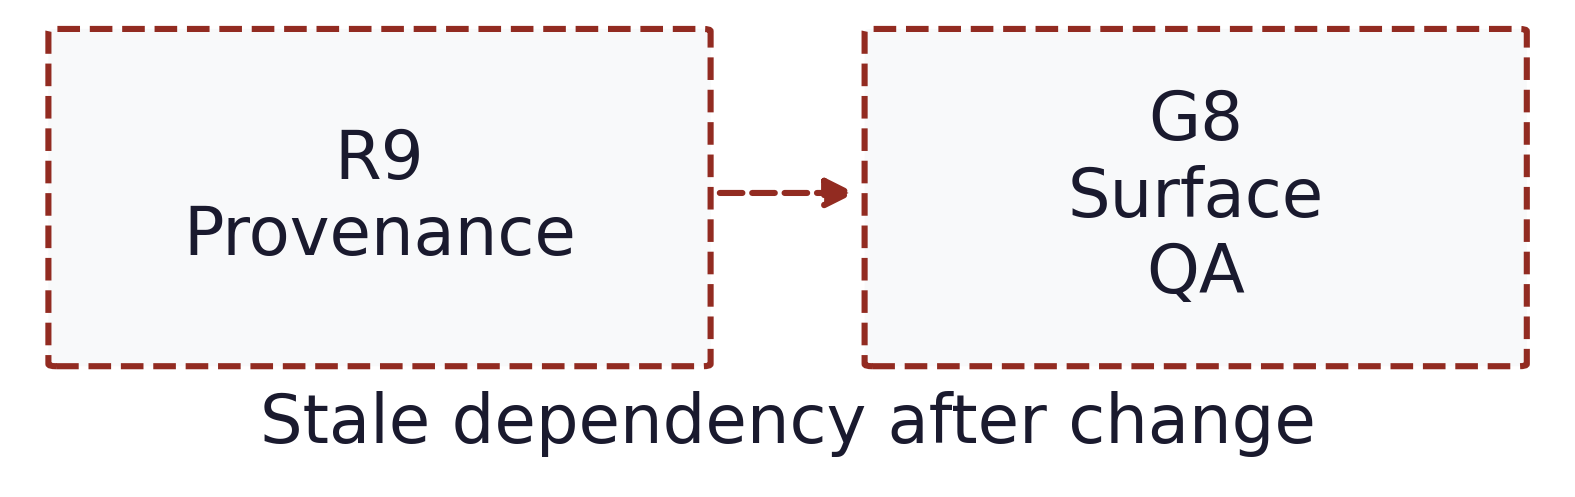
\includegraphics[keepaspectratio,width=0.98\linewidth,height=0.8\textheight,alt={R9 Provenance → G8 Surface QA: Stale dependency after change; invalidation.}]{../figures/source_render_provenance.slide-invalidation-surface-validation-provenance.png}
\refstepcounter{figure}\label{fig:source-render-provenance-slide-panel-50}
\end{figure}
\end{frame}

\begin{frame}{Producer order, stale\ldots{} (part 57)}
\begin{figure}
\centering
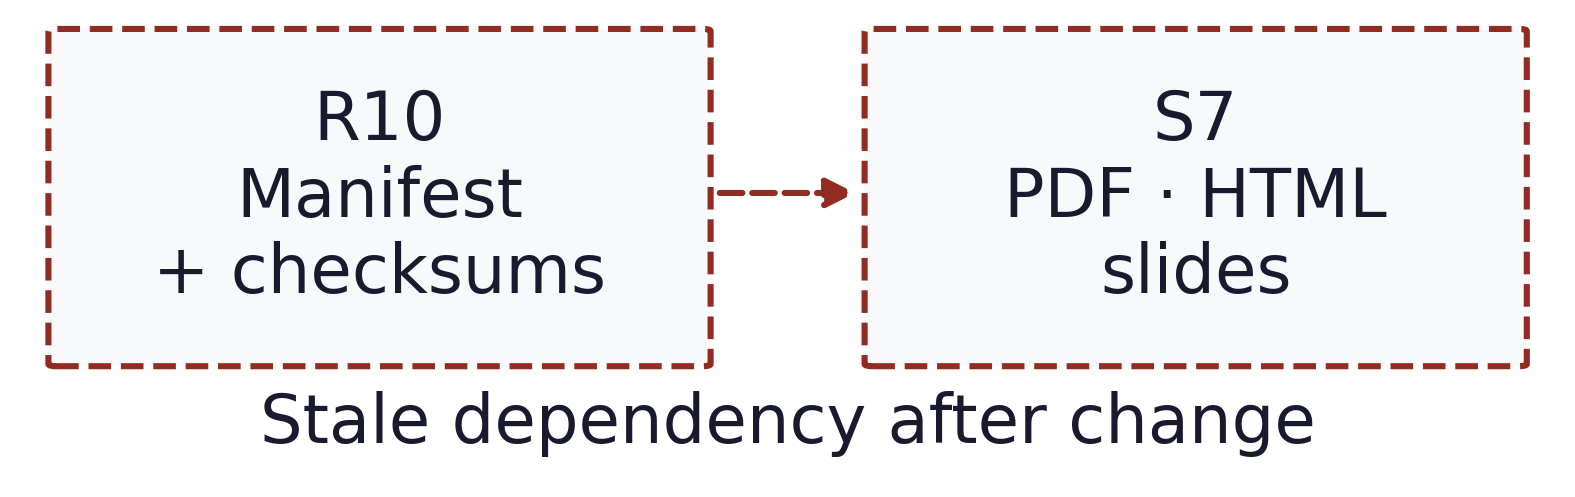
\includegraphics[keepaspectratio,width=0.98\linewidth,height=0.8\textheight,alt={R10 Manifest + checksums → S7 PDF · HTML slides: Stale dependency after change; invalidation.}]{../figures/source_render_provenance.slide-invalidation-surfaces-release-manifest.png}
\refstepcounter{figure}\label{fig:source-render-provenance-slide-panel-51}
\end{figure}
\end{frame}

\begin{frame}{Producer order, stale\ldots{} (part 58)}
\begin{figure}
\centering
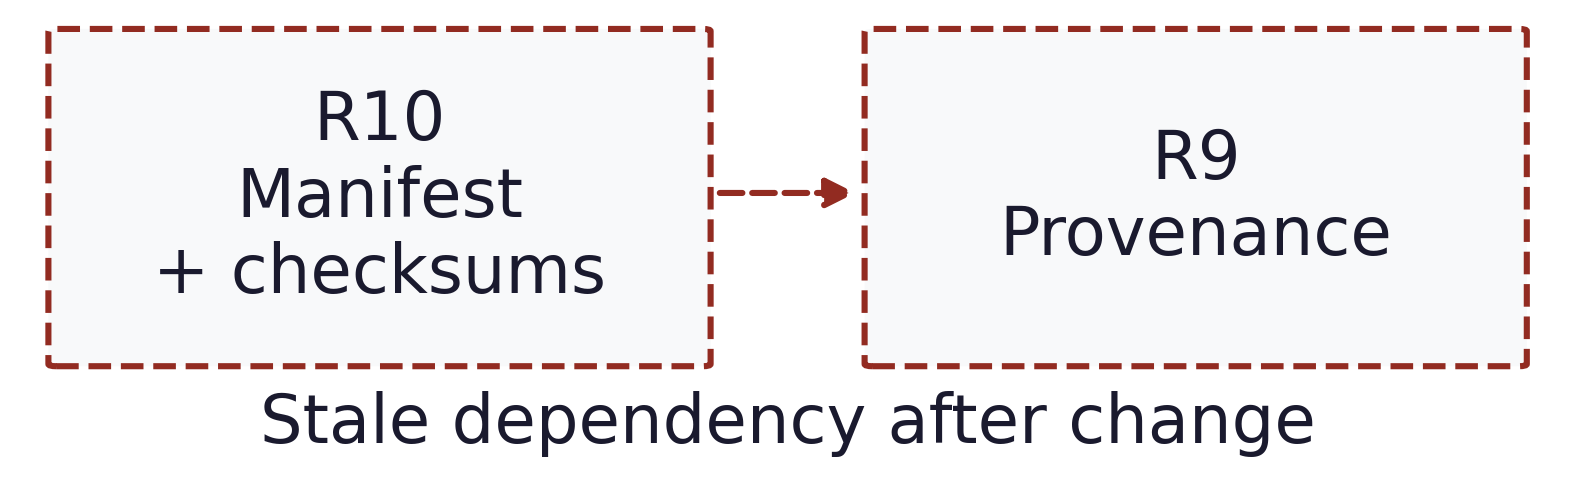
\includegraphics[keepaspectratio,width=0.98\linewidth,height=0.8\textheight,alt={R10 Manifest + checksums → R9 Provenance: Stale dependency after change; invalidation.}]{../figures/source_render_provenance.slide-invalidation-provenance-release-manifest.png}
\refstepcounter{figure}\label{fig:source-render-provenance-slide-panel-52}
\end{figure}
\end{frame}

\begin{frame}{Producer order, stale\ldots{} (part 59)}
\begin{figure}
\centering
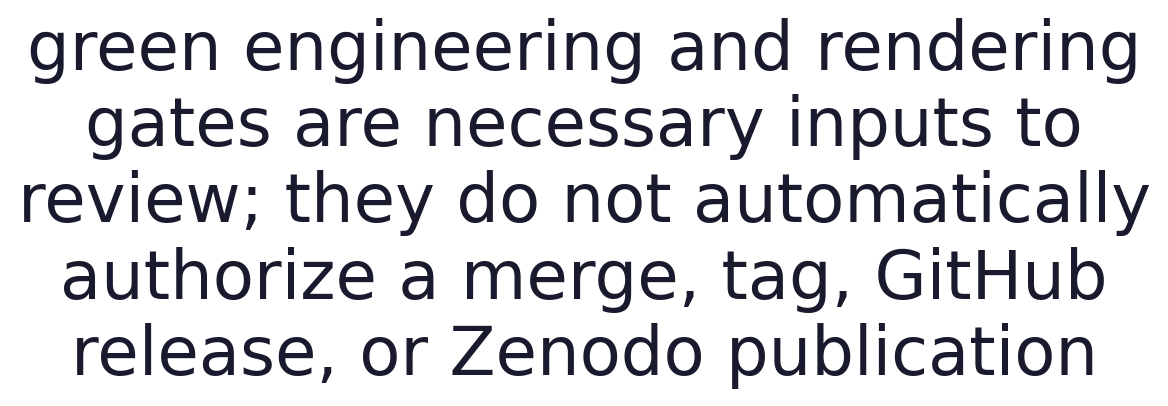
\includegraphics[keepaspectratio,width=0.98\linewidth,height=0.8\textheight,alt={green engineering and rendering gates are necessary inputs to review; they do not automatically authorize a merge, tag, GitHub release, or Zenodo publication}]{../figures/source_render_provenance.slide-authorization-boundary.png}
\refstepcounter{figure}\label{fig:source-render-provenance-slide-panel-53}
\end{figure}
\end{frame}

\begin{frame}{Producer order, stale\ldots{} (part 60)}
\begin{figure}
\centering
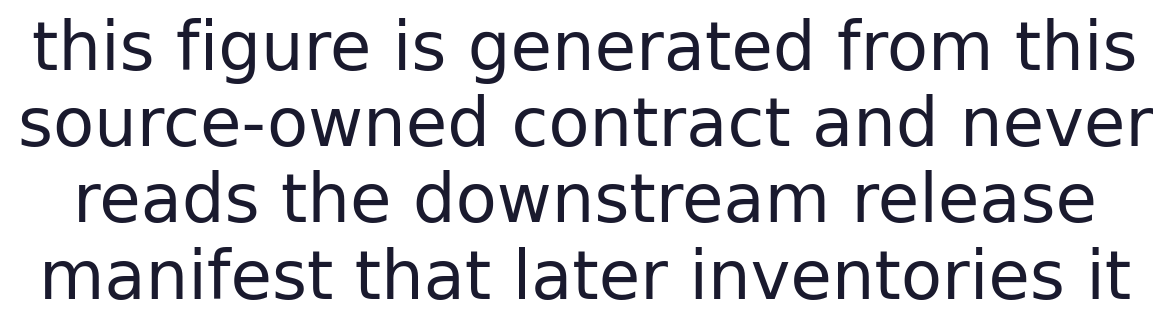
\includegraphics[keepaspectratio,width=0.98\linewidth,height=0.8\textheight,alt={this figure is generated from this source-owned contract and never reads the downstream release manifest that later inventories it}]{../figures/source_render_provenance.slide-manifest-cycle-boundary.png}
\refstepcounter{figure}\label{fig:source-render-provenance-slide-panel-54}
\end{figure}
\end{frame}

\begin{frame}{Producer order, stale\ldots{} (part 61)}
\begin{figure}
\centering

\includegraphics[keepaspectratio,width=0.98\linewidth,height=0.8\textheight,alt={a green build is not scientific validation}]{../figures/source_render_provenance.slide-no-claim-1.png}
\refstepcounter{figure}\label{fig:source-render-provenance-slide-panel-55}
\end{figure}
\end{frame}

\begin{frame}{Producer order, stale\ldots{} (part 62)}
\begin{figure}
\centering

\includegraphics[keepaspectratio,width=0.98\linewidth,height=0.8\textheight,alt={tagged PDF structure is not PDF/UA conformance}]{../figures/source_render_provenance.slide-no-claim-2.png}
\refstepcounter{figure}\label{fig:source-render-provenance-slide-panel-56}
\end{figure}
\end{frame}

\begin{frame}{Producer order, stale\ldots{} (part 63)}
\begin{figure}
\centering

\includegraphics[keepaspectratio,width=0.98\linewidth,height=0.8\textheight,alt={HTML accessibility enhancements are not a WCAG conformance claim}]{../figures/source_render_provenance.slide-no-claim-3.png}
\refstepcounter{figure}\label{fig:source-render-provenance-slide-panel-57}
\end{figure}
\end{frame}

\begin{frame}{Producer order, stale\ldots{} (part 64)}
\begin{figure}
\centering

\includegraphics[keepaspectratio,width=0.98\linewidth,height=0.8\textheight,alt={a GitHub release or DOI does not enlarge the scientific claim surface}]{../figures/source_render_provenance.slide-no-claim-4.png}
\refstepcounter{figure}\label{fig:source-render-provenance-slide-panel-58}
\end{figure}
\end{frame}

\begin{frame}{Recovery-limit certificate for the client and project-pool
corners}
\protect\phantomsection\label{sec:repro-recovery}
The recovery identities are reproducibility checks: the client machinery
must return to standard Bayes at its KL/NLL loss limits,
\end{frame}

\begin{frame}{Recovery-limit certificate\ldots{} (part 2)}
and the server heuristic must return to the project's log-linear pool at
zero robustness (eq.~10,
eq.~11).
\end{frame}

\begin{frame}{Recovery-limit certificate\ldots{} (part 3)}
Under the explicit shared-support, posterior-log-potential, and
fixed-weight assumptions of sec.~5.8, that pool
specializes Eq. 7's message-combination term; it does not reproduce the
complete source protocol. These deviations are computed on every build.
\end{frame}

\begin{frame}[fragile]{Recovery-limit certificate\ldots{} (part 4)}
\textbf{Server recovery:} \texttt{robust\_aggregate(robustness=0)}
versus \texttt{log\_linear\_pool} (eq.~9) has
maximum difference 0.
\end{frame}

\begin{frame}[fragile]{Recovery-limit certificate\ldots{} (part 5)}
\textbf{Posterior recovery:} \texttt{generalized\_posterior(KLD,\ NLL)}
versus closed-form Bayes has maximum difference 5.55e-17.

\textbf{Divergence recovery:} Rényi divergence versus KL as
\(\alpha\to 1\) has maximum difference 0.
\end{frame}

\begin{frame}{Recovery-limit certificate\ldots{} (part 6)}
\textbf{Loss recoveries:} \(\beta\)-loss versus NLL as \(\beta\to 0\)
has maximum difference 0, while rcce versus NLL as
\(q_{\text{loss}}\to 0\) has maximum difference 0.
\end{frame}

\begin{frame}{Recovery-limit certificate\ldots{} (part 7)}
Any drift in these limits beyond machine precision would mean the robust
generalization no longer contains its standard-Bayes client limit and
project-local log-linear-pool server limit
(sec.~7.1) --- and would fail the core test suite
before this certificate could render.
\end{frame}

\begin{frame}[fragile]{Recovery-limit certificate\ldots{} (part 8)}
The certificate covers the recovery identity and the client-side result
under the cited source theorem's matching assumptions only; the
server-side \texttt{robust\_aggregate} heuristic is certified here for
its recovery limit alone, not for any bounded-influence property
(sec.~8.13).
\end{frame}

\begin{frame}{Recovery-limit certificate\ldots{} (part 9)}
All code is authored by Daniel Ari Friedman and licensed under the MIT
license. This is project version 1.1.0.
\end{frame}

\end{document}
